%===========================================================
\postextualchapter{Efficiency maps}\label{app:efficiencies}
%===========================================================

All the Efficiency maps are used for the efficiency calculation, as explained in Sec. \ref{sec:efficiency}, are displayed here.

\section{Efficiencies for sample 2016APV}

\begin{figure}[H]{15cm}
  \caption{$\Upsilon$ acceptance of the selected associated $\Upsilon +$ D$^*$ extracted from 2016APV MC sample.}
  \label{fig:acc_dimu_2016APV}
  \subfloat[][]{\label{subfig:acc_dimu_pt_2016APV}%
    \fbox{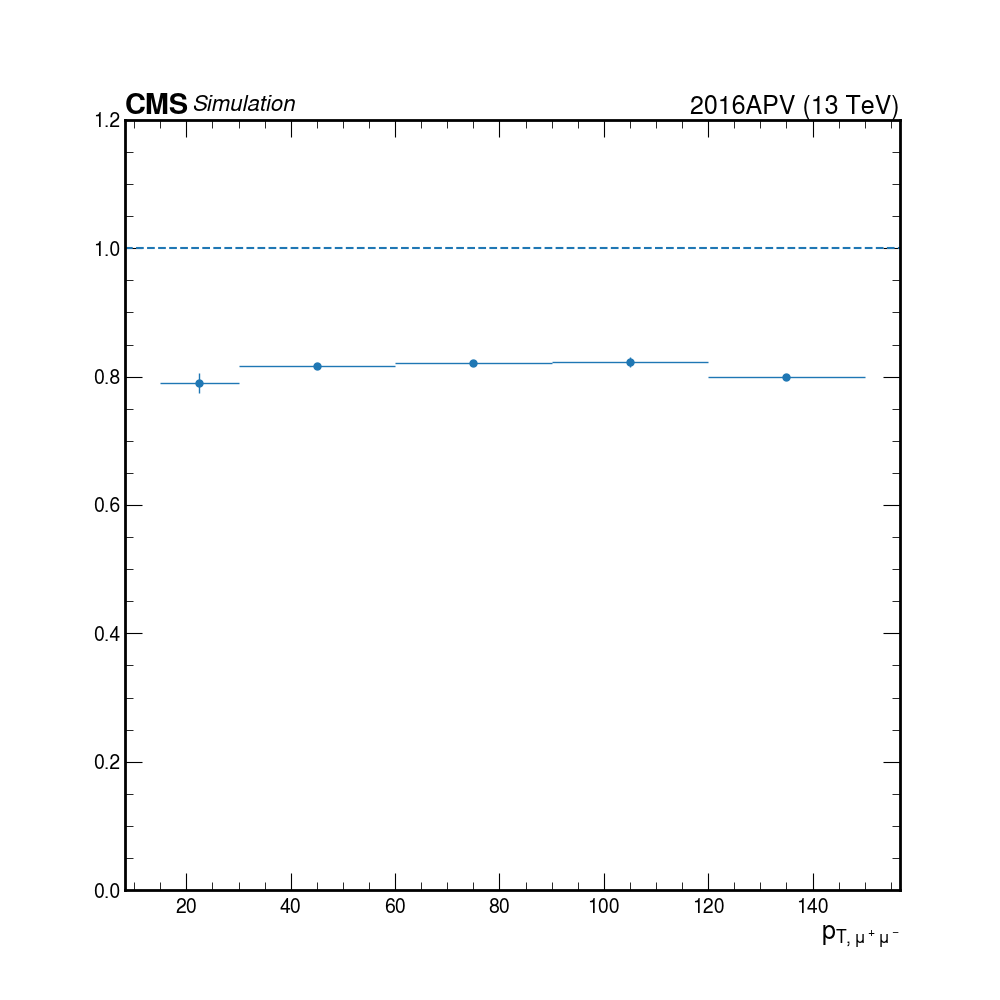
\includegraphics[width=0.44\textwidth]{figures/efficiency/acc_dimu_pt_2016APV.png}}}\hfill
  \subfloat[][]{\label{subfig:acc_dimu_rap_2016APV}%
    \fbox{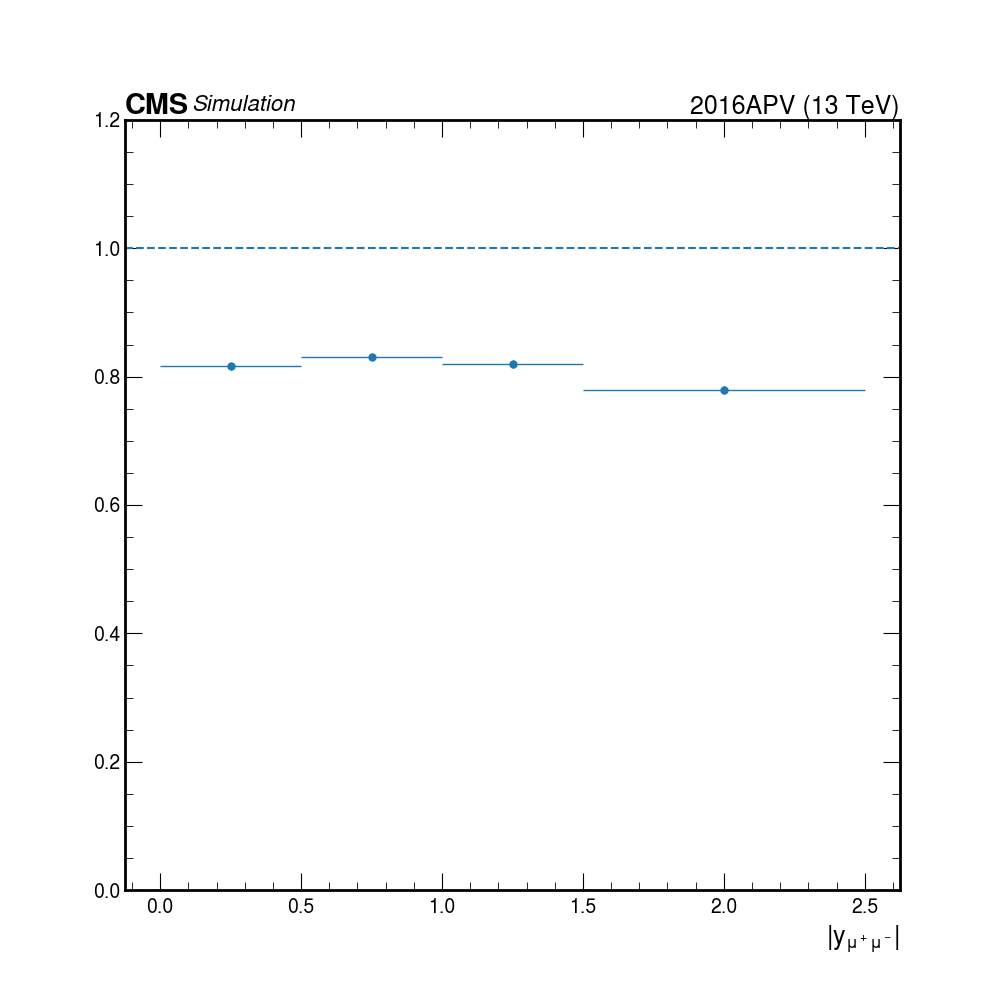
\includegraphics[width=0.44\textwidth]{figures/efficiency/acc_dimu_rap_2016APV.png}}}\hfill\\
  \subfloat[][]{\label{subfig:acc_dimu_2D_2016APV}%
    \fbox{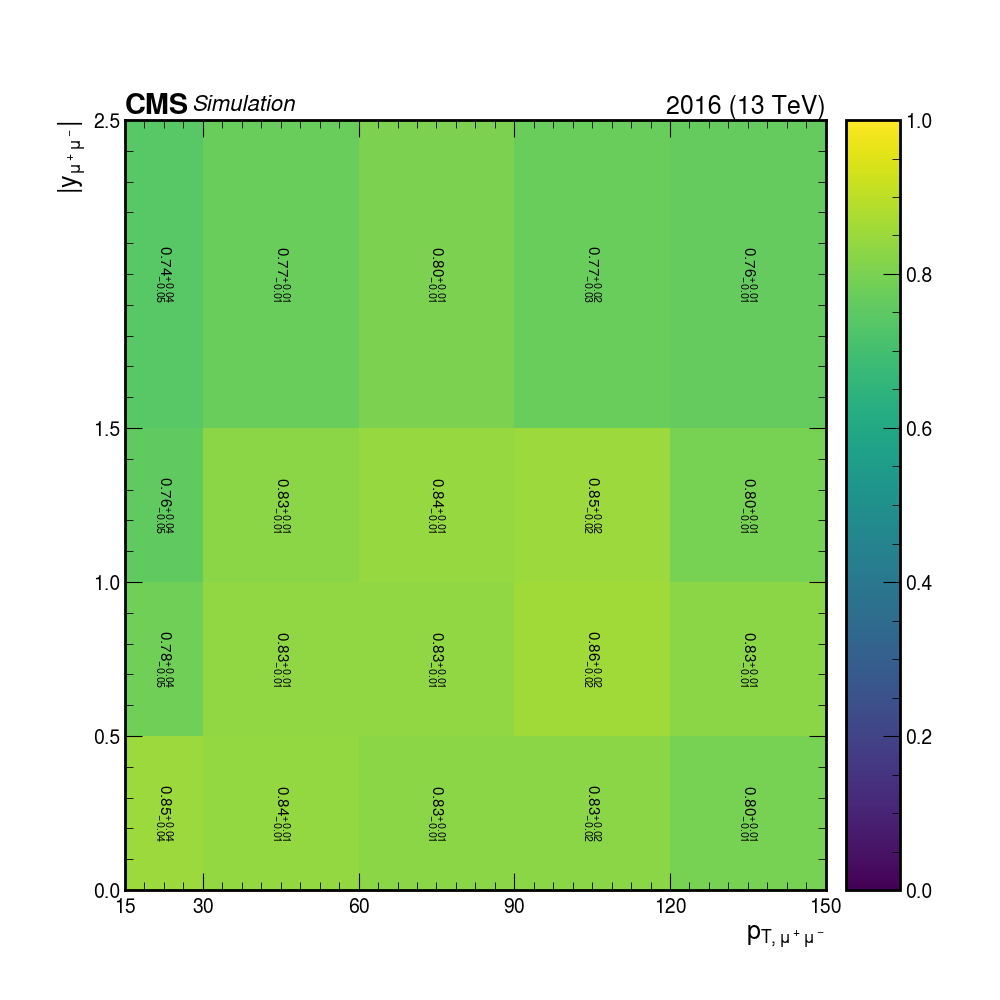
\includegraphics[width=0.44\textwidth]{figures/efficiency/acc_dimu_2016APV.png}}}\\
  \legend{$\Upsilon$ acceptance extracted from the 2016APV MC data sample. The acceptance is given with respect to the dimuon $p_T$ in (a), $y$ in (b), and in both $p_T$ and $y$ in (c). In (a) and (b). The horizontal dashed line is set to the upper limit of the acceptance, one.}
\end{figure}

\begin{figure}[H]{15cm}
  \caption{D$^*$ acceptance of the selected associated $\Upsilon +$ D$^*$ extracted from 2016APV MC sample.}
  \label{fig:acc_dstar_2016APV}
  \subfloat[][]{\label{subfig:acc_dstar_pt_2016APV}%
    \fbox{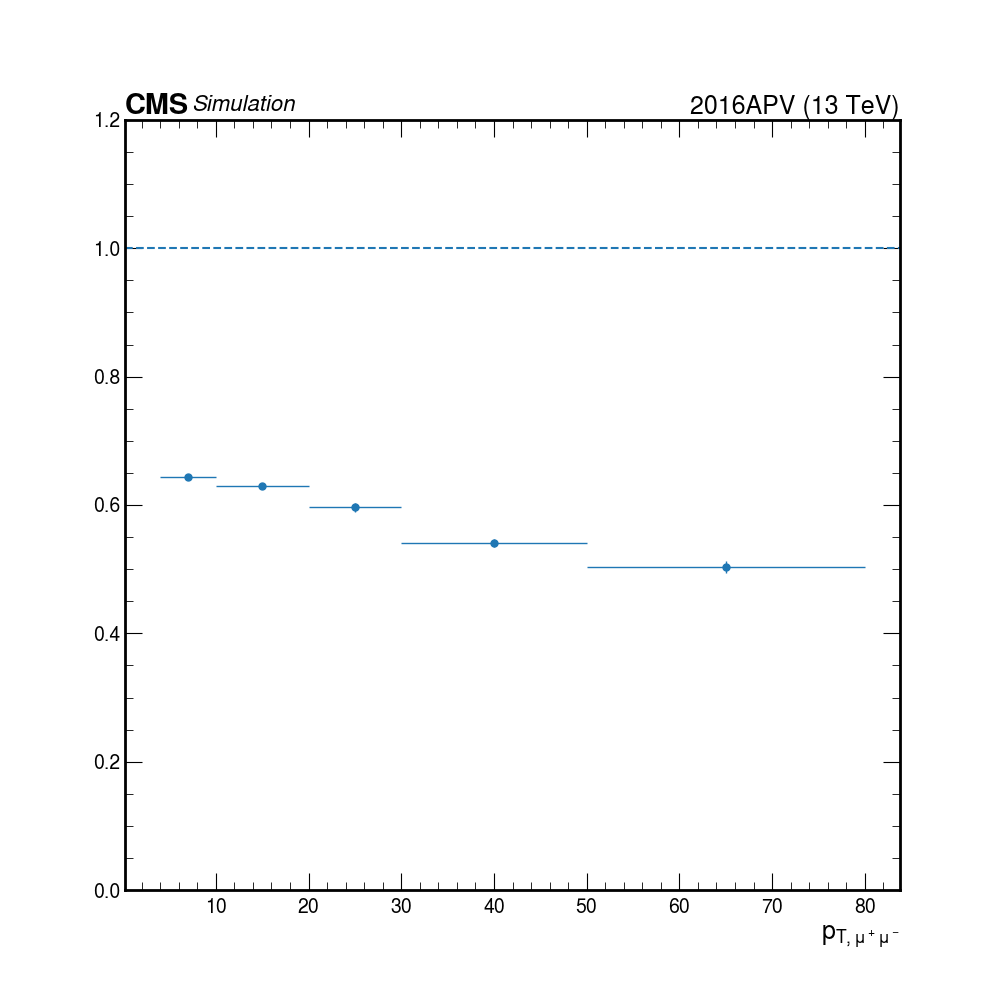
\includegraphics[width=0.44\textwidth]{figures/efficiency/acc_dstar_pt_2016APV.png}}}\hfill
  \subfloat[][]{\label{subfig:acc_dstar_rap_2016APV}%
    \fbox{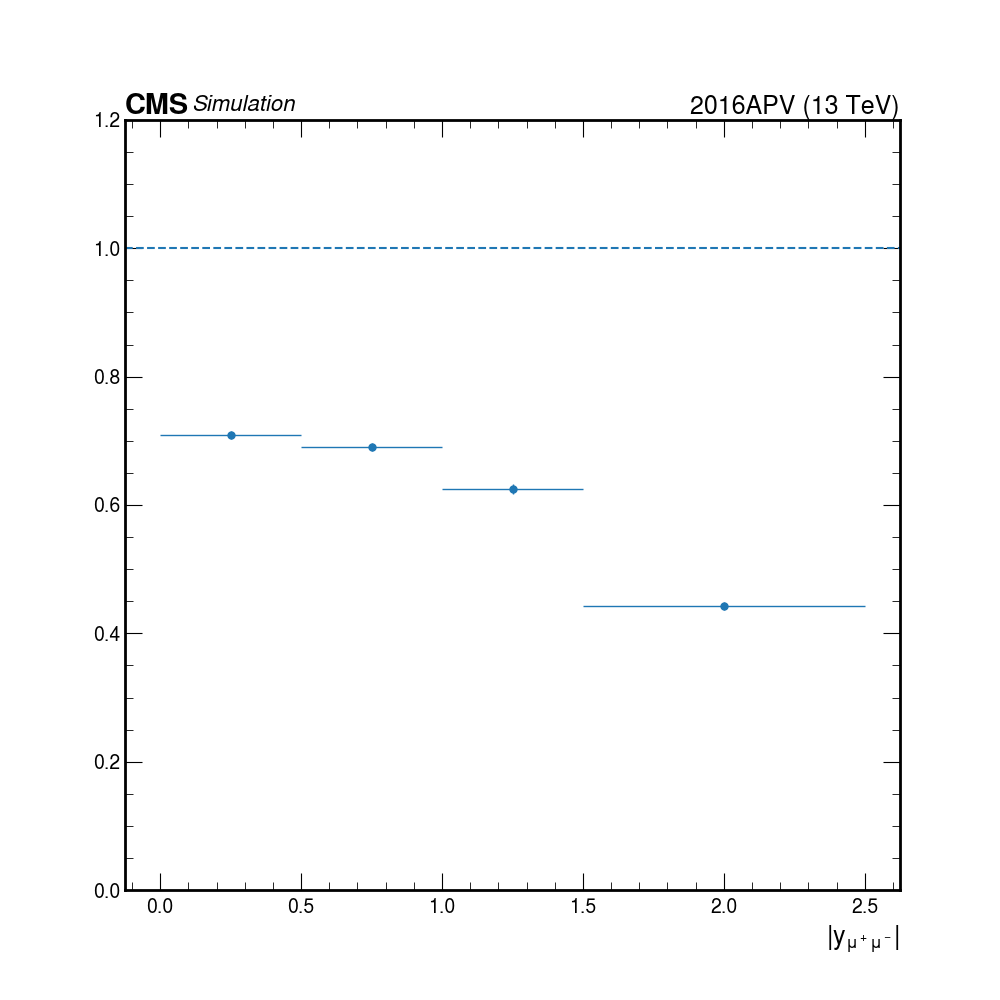
\includegraphics[width=0.44\textwidth]{figures/efficiency/acc_dstar_rap_2016APV.png}}}\hfill\\
  \subfloat[][]{\label{subfig:acc_dstar_2D_2016APV}%
    \fbox{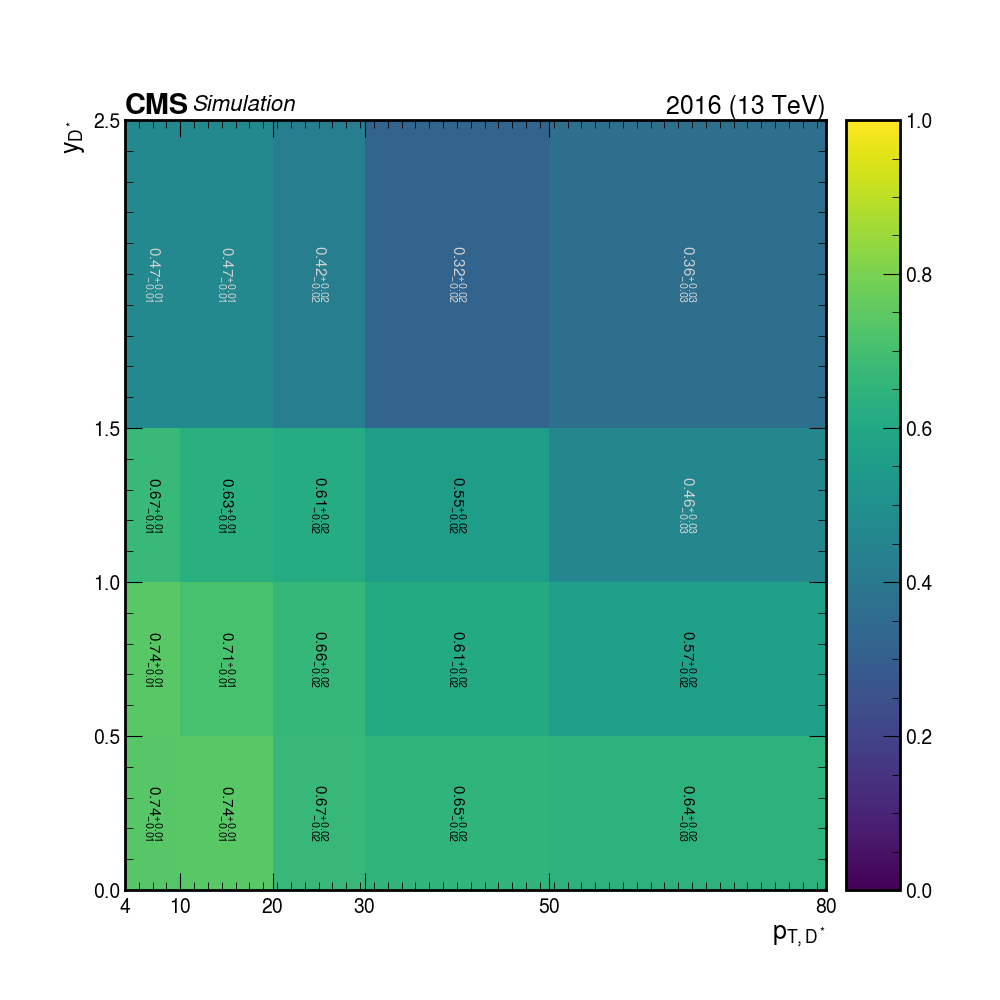
\includegraphics[width=0.44\textwidth]{figures/efficiency/acc_dstar_2016APV.png}}}\\
  \legend{D$^*$ acceptance extracted from the 2016APV MC data sample. The acceptance is given with respect to the reconstructed D$^*$ $p_T$ in (a), $y$ in (b), and in both $p_T$ and $y$ in (c). In (a) and (b). The horizontal dashed line is set to the upper limit of the acceptance, one.}
\end{figure}

\begin{figure}[H]{15cm}
  \caption{$\Upsilon$ selection cuts efficiency of the selected associated $\Upsilon +$ D$^*$ extracted from 2016APV MC sample.}
  \label{fig:eff_cuts_dimu_2016APV}
  \subfloat[][]{\label{subfig:eff_cuts_dimu_pt_2016APV}%
  \fbox{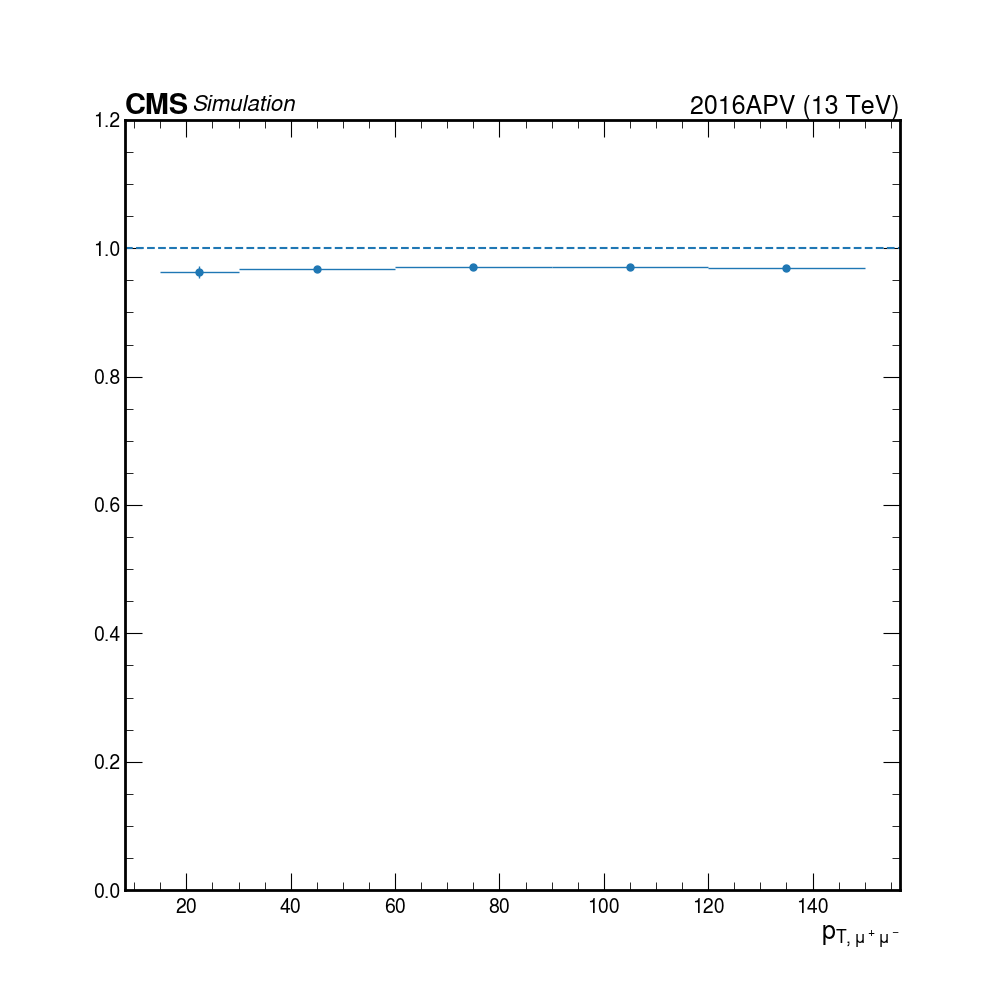
\includegraphics[width=0.44\textwidth]{figures/efficiency/eff_cuts_dimu_pt_2016APV.png}}}\hfill
  \subfloat[][]{\label{subfig:eff_cuts_dimu_rap_2016APV}%
  \fbox{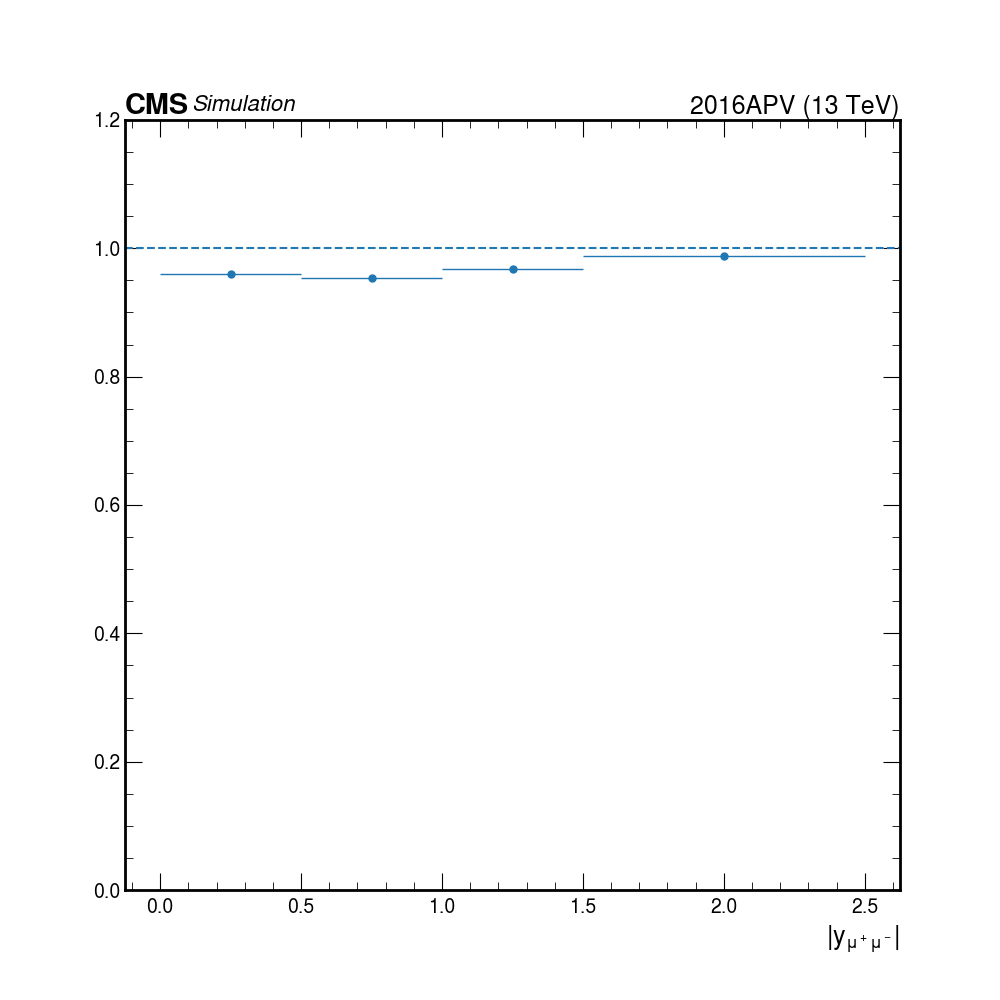
\includegraphics[width=0.44\textwidth]{figures/efficiency/eff_cuts_dimu_rap_2016APV.png}}}\hfill\\
  \subfloat[][]{\label{subfig:eff_cuts_dimu_2D_2016APV}%
  \fbox{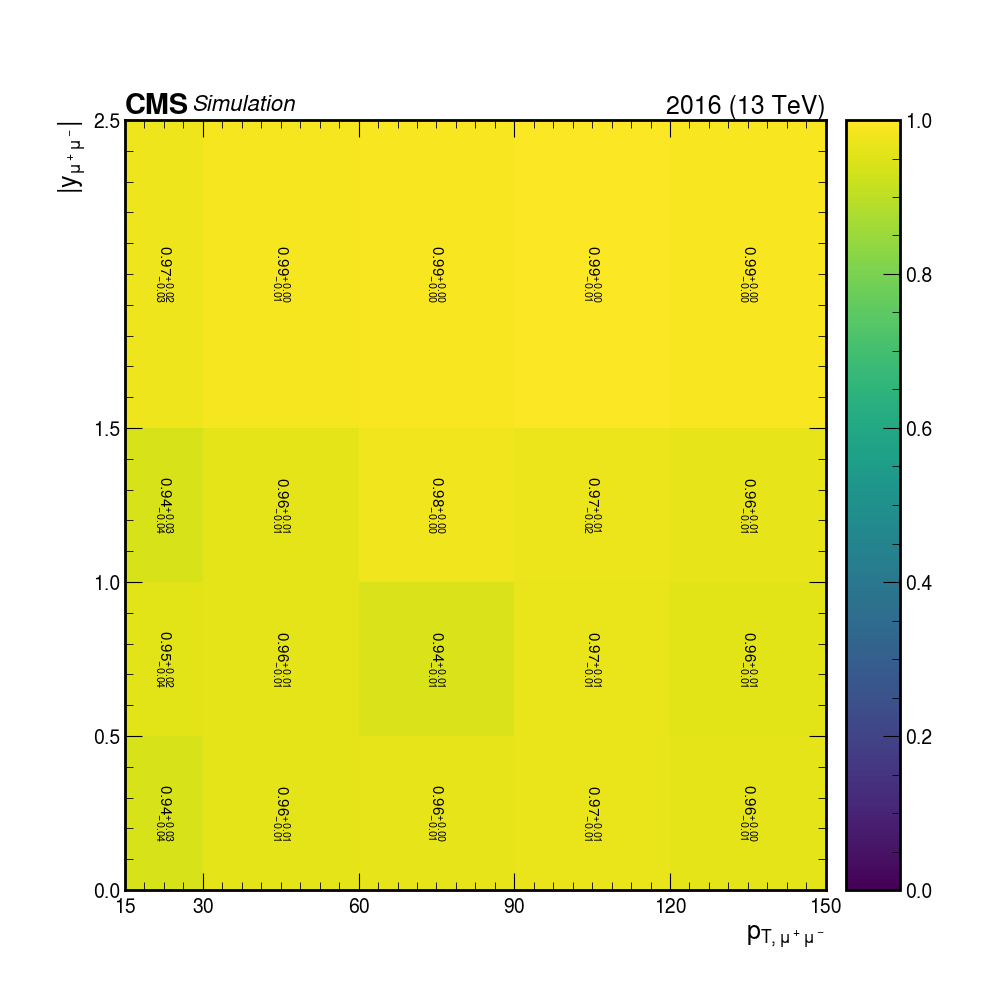
\includegraphics[width=0.44\textwidth]{figures/efficiency/eff_cuts_dimu_2016APV.png}}}\\
  \legend{$\Upsilon$ selection cuts efficiency extracted from the 2016APV MC data sample. This efficiency is given with respect to the dimuon $p_T$ in (a), $y$ in (b), and in both $p_T$ and $y$ in (c). In (a) and (b). The horizontal dashed line is set to the upper limit of the efficiency.}
\end{figure}

\begin{figure}[H]{15cm}
  \caption{D$^*$ selection cuts efficiency of the selected associated $\Upsilon +$ D$^*$ extracted from 2016APV MC sample.}
  \label{fig:eff_cuts_dstar_2016APV}
  \subfloat[][]{\label{subfig:eff_cuts_dstar_pt_2016APV}%
    \fbox{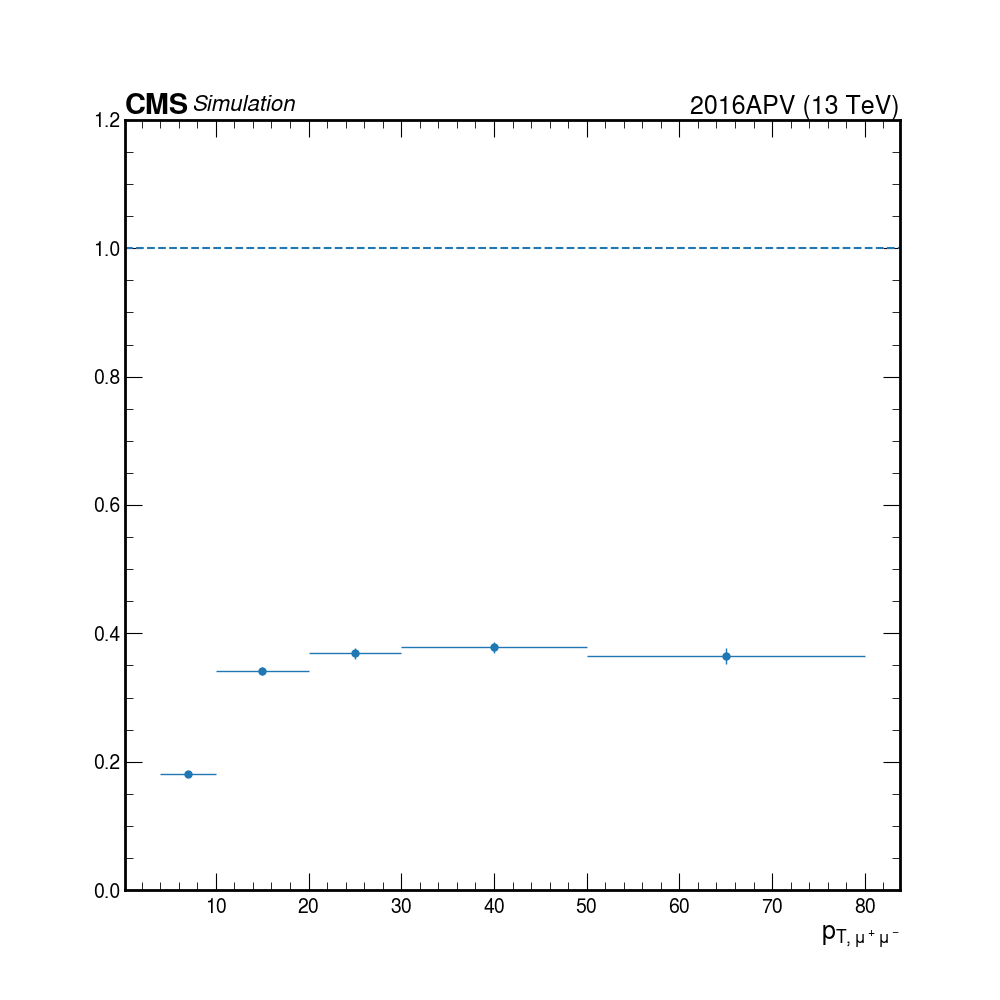
\includegraphics[width=0.44\textwidth]{figures/efficiency/eff_cuts_dstar_pt_2016APV.png}}}\hfill
  \subfloat[][]{\label{subfig:eff_cuts_dstar_rap_2016APV}%
    \fbox{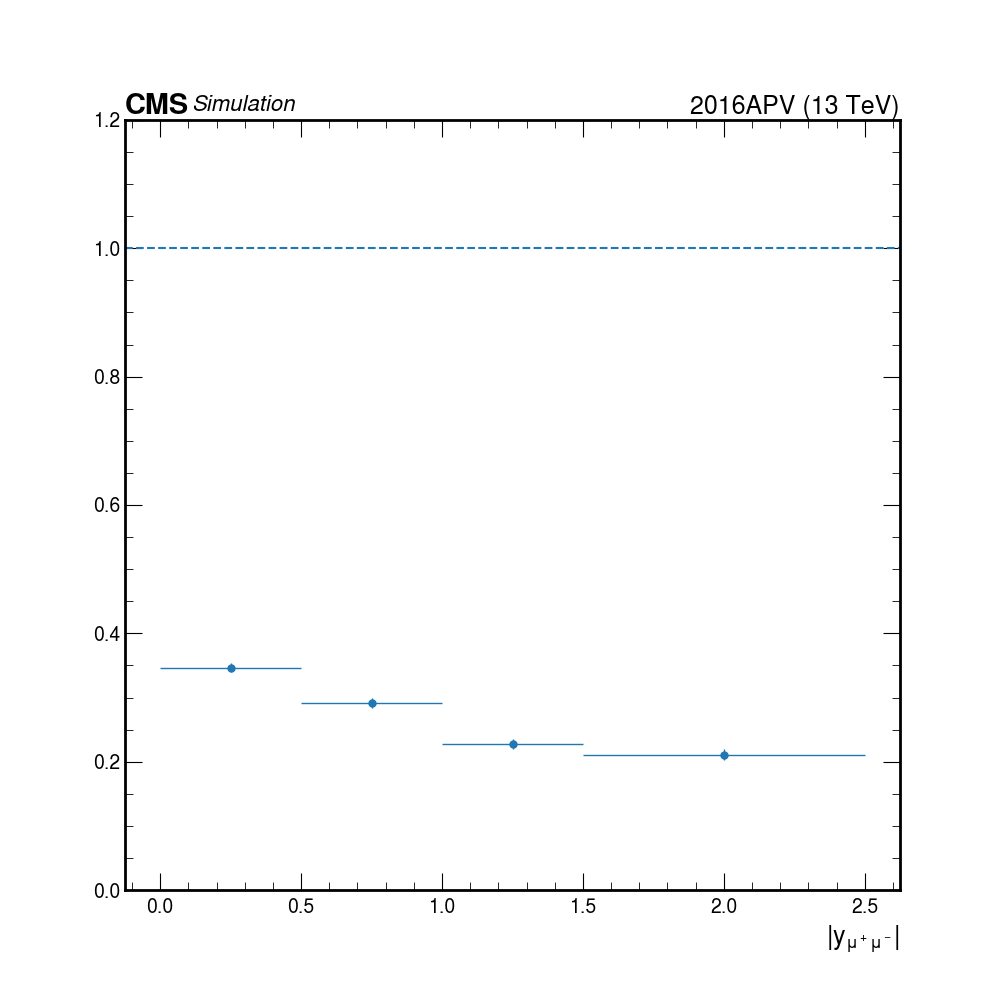
\includegraphics[width=0.44\textwidth]{figures/efficiency/eff_cuts_dstar_rap_2016APV.png}}}\hfill\\
  \subfloat[][]{\label{subfig:eff_cuts_dstar_2D_2016APV}%
    \fbox{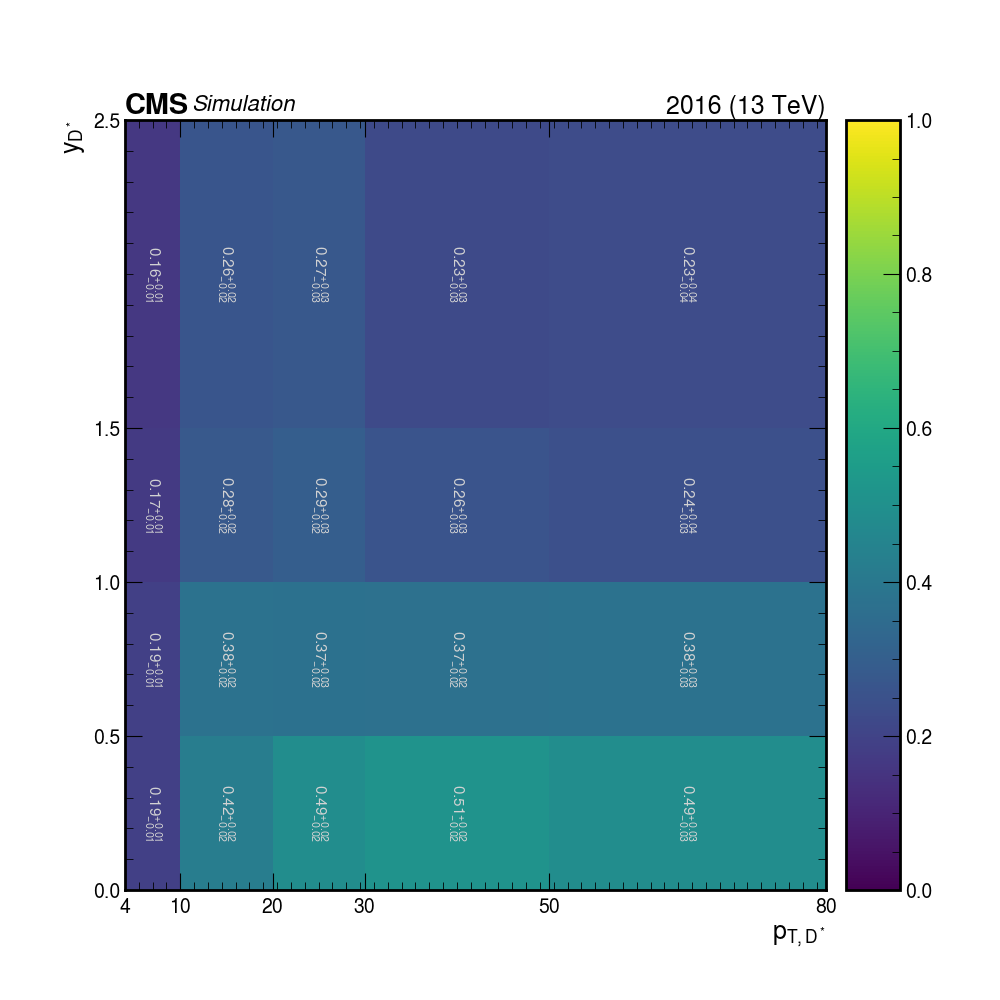
\includegraphics[width=0.44\textwidth]{figures/efficiency/eff_cuts_dstar_2016APV.png}}}\\
  \legend{D$^*$ selection cuts efficiency extracted from the 2016APV MC data sample. This efficiency is given with respect to the D$^*$ $p_T$ in (a), $y$ in (b), and in both $p_T$ and $y$ in (c). In (a) and (b). The horizontal dashed line is set to the upper limit of the efficiency.}
\end{figure}

\begin{figure}[H]{15cm}
  \caption{Trigger efficiency of the selected associated $\Upsilon +$ D$^*$ extracted from 2016APV MC sample.}
  \label{fig:eff_trigger_2016APV}
  \subfloat[][]{\label{subfig:eff_trigger_pt_2016APV}%
    \fbox{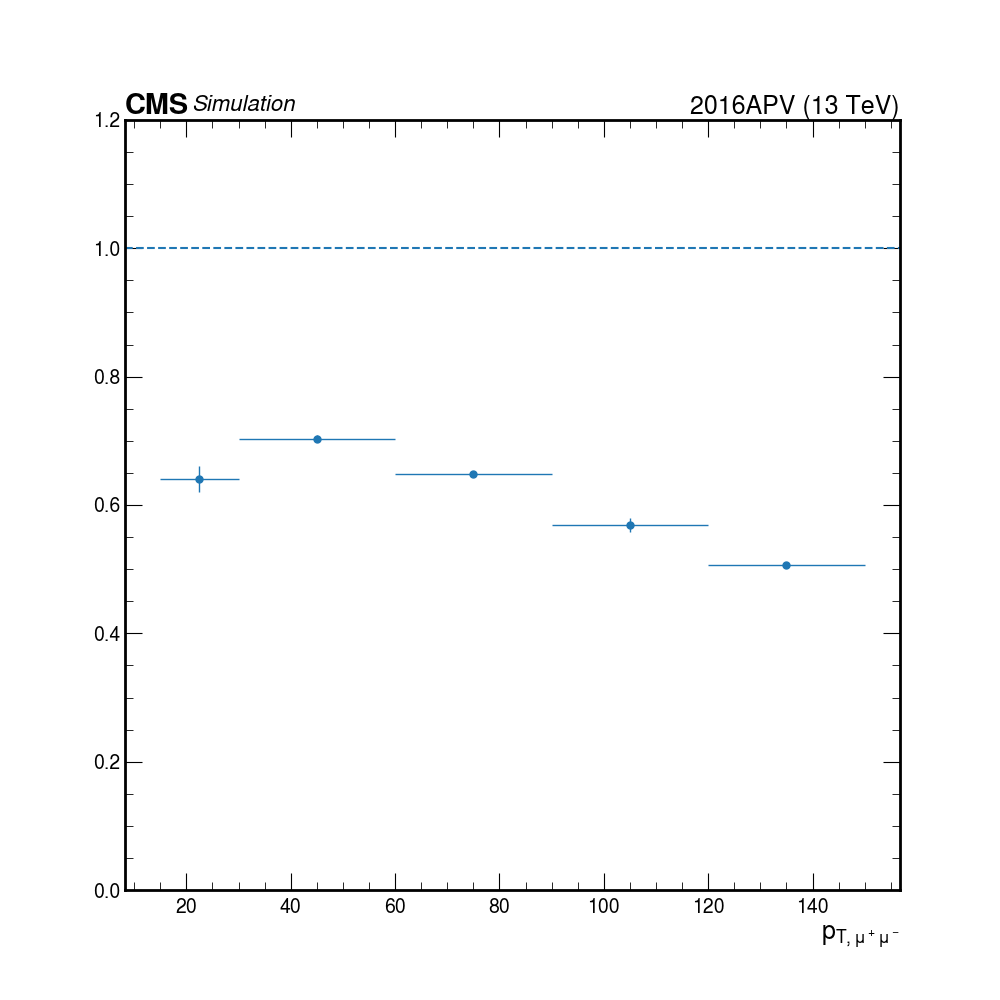
\includegraphics[width=0.44\textwidth]{figures/efficiency/eff_trigger_pt_2016APV.png}}}\hfill
  \subfloat[][]{\label{subfig:eff_trigger_rap_2016APV}%
    \fbox{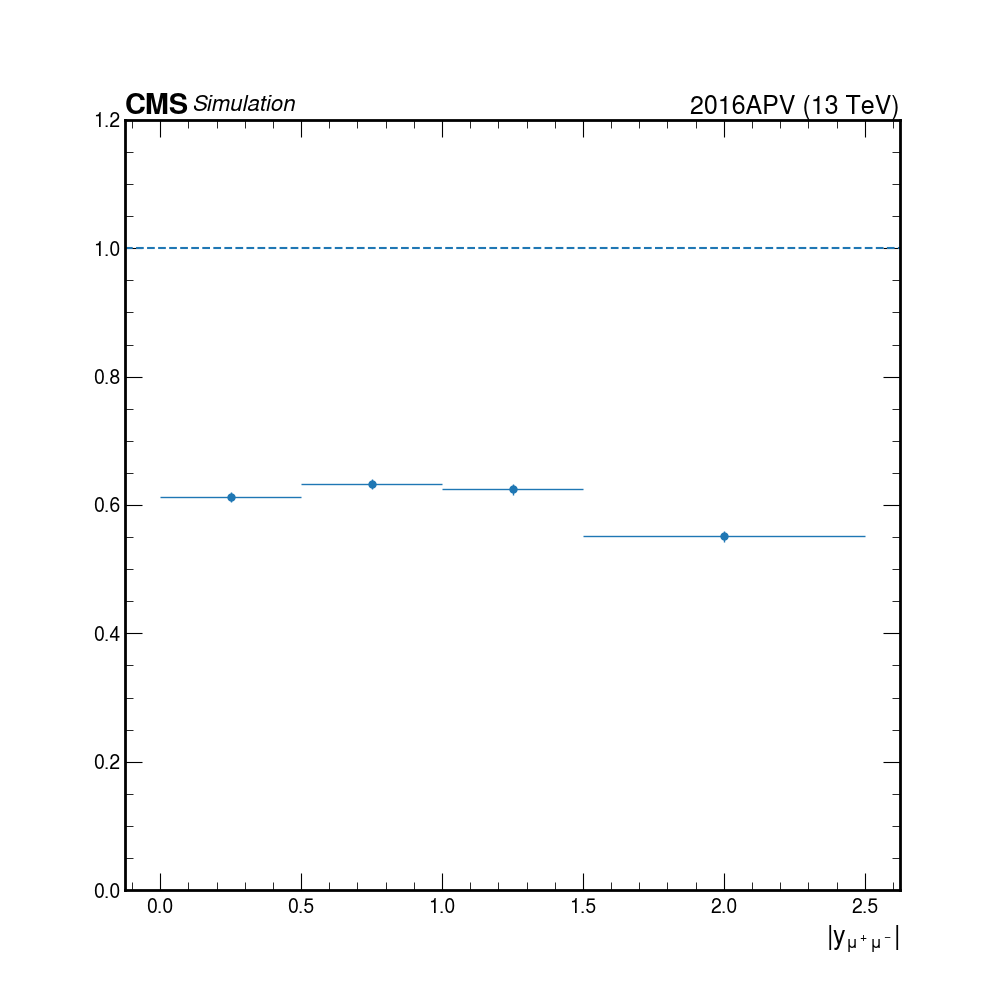
\includegraphics[width=0.44\textwidth]{figures/efficiency/eff_trigger_rap_2016APV.png}}}\hfill\\
  \subfloat[][]{\label{subfig:eff_trigger_2D_2016APV}%
    \fbox{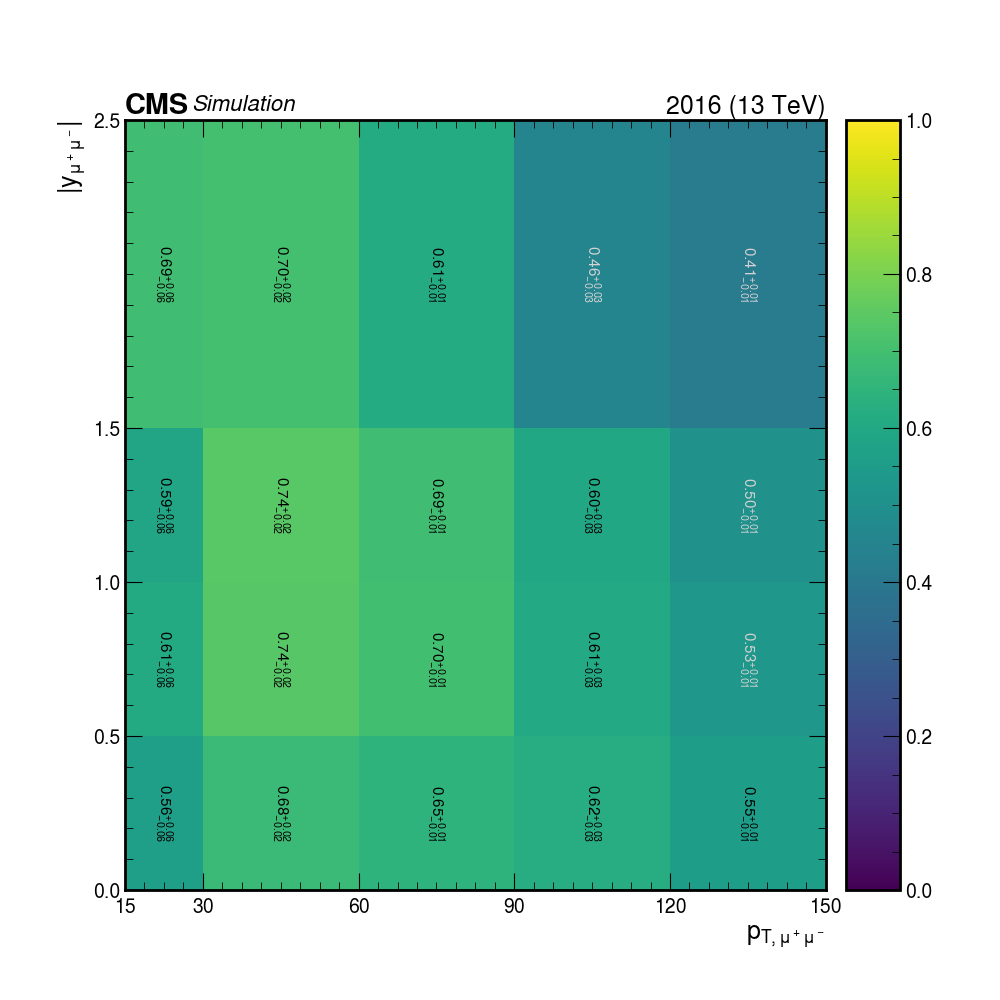
\includegraphics[width=0.44\textwidth]{figures/efficiency/eff_trigger_2016APV.png}}}\\
  \legend{Trigger efficiency extracted from the 2016APV MC data sample. This efficiency is given with respect to the dimuon $p_T$ in (a), $y$ in (b), and in both $p_T$ and $y$ in (c). In (a) and (b). The horizontal dashed line is set to the upper limit of the efficiency.}
\end{figure}

\begin{figure}[H]{15cm}
  \caption{Trigger efficiency of the selected associated $\Upsilon +$ D$^*$ extracted from 2016APV MC sample.}
  \label{fig:eff_asso_2016APV}
  \subfloat[][]{\label{subfig:eff_asso_pt_2016APV}%
    \fbox{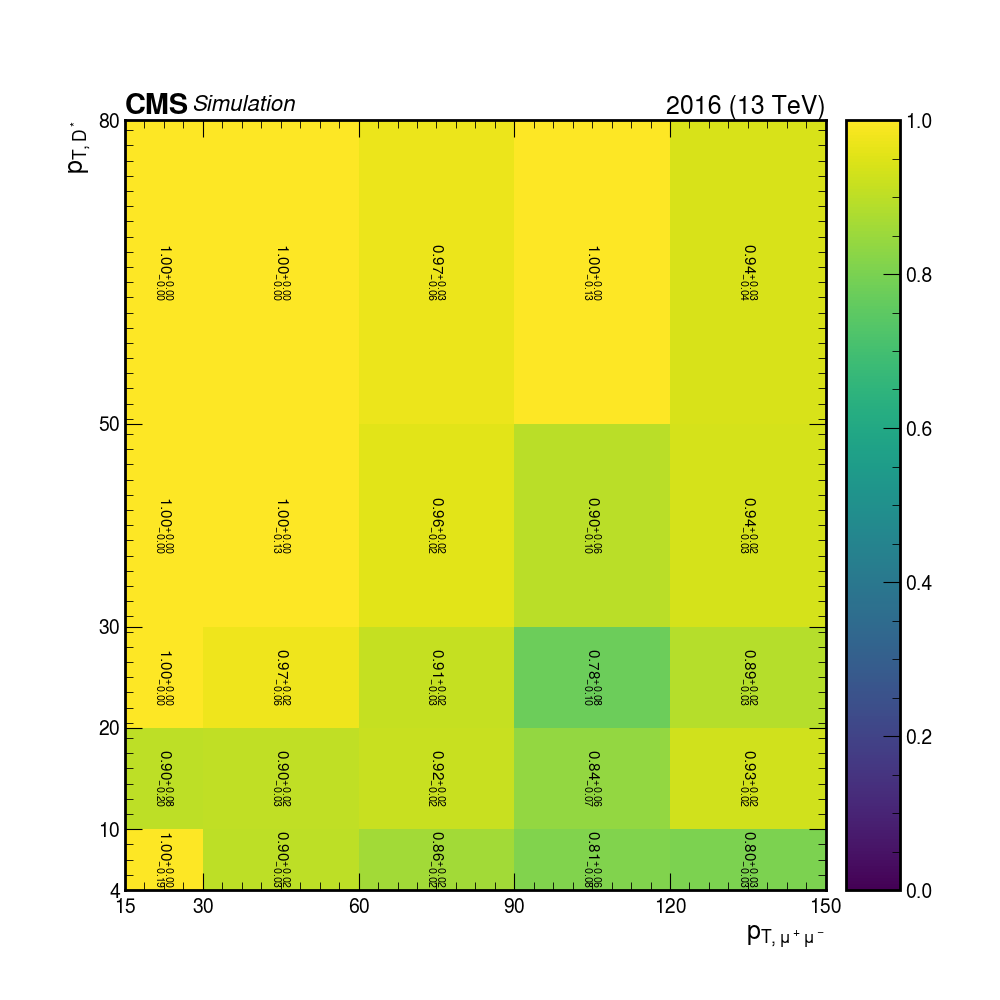
\includegraphics[width=0.44\textwidth]{figures/efficiency/eff_asso_pt_2016APV.png}}}\hfill
  \subfloat[][]{\label{subfig:eff_asso_rap_2016APV}%
    \fbox{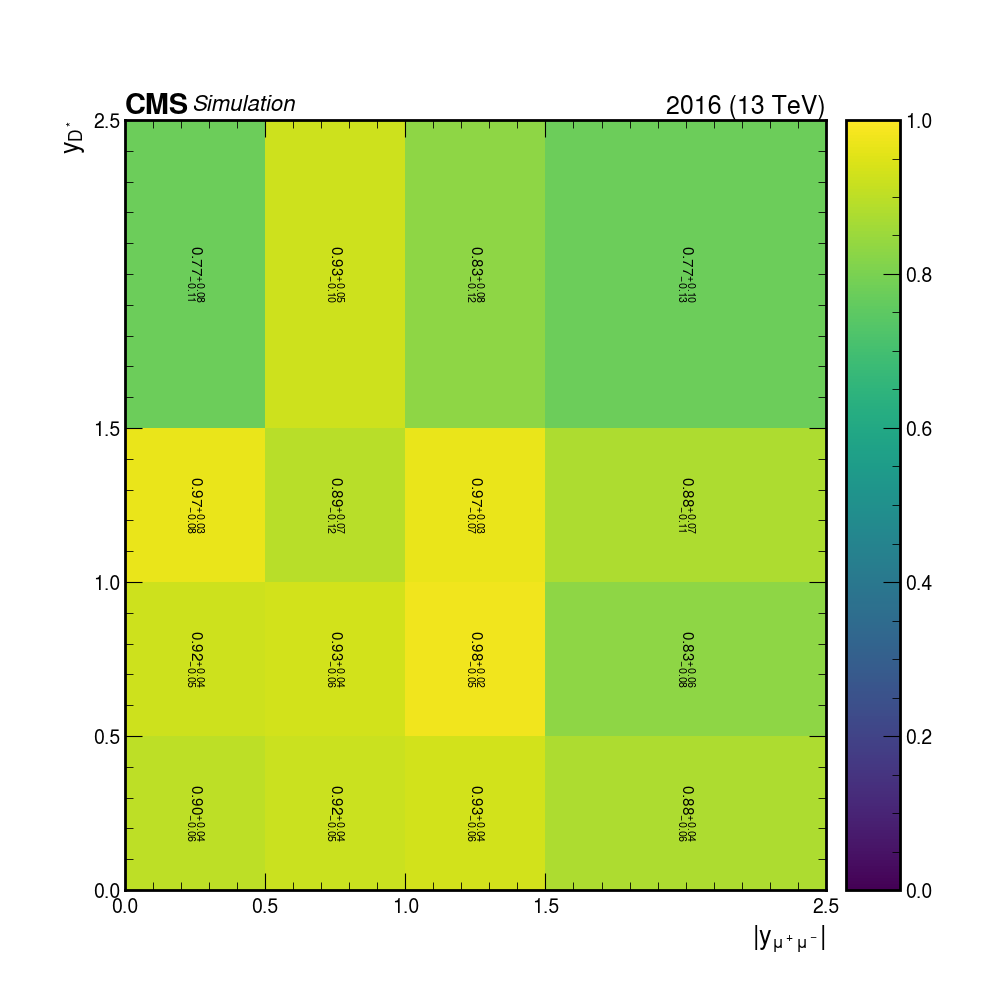
\includegraphics[width=0.44\textwidth]{figures/efficiency/eff_asso_rap_2016APV.png}}}\hfill\\
  \legend{Association efficiency extracted from the 2016APV MC data sample. The efficiency maps are given with respect to the dimuon and D$^*$ $p_T$ in (a) and $y$ in (b).}
\end{figure}

\clearpage

\section{Efficiencies for sample 2016}

\begin{figure}[H]{15cm}
  \caption{$\Upsilon$ acceptance of the selected associated $\Upsilon +$ D$^*$ extracted from 2016 MC sample.}
  \label{fig:acc_dimu_2016}
  \subfloat[][]{\label{subfig:acc_dimu_pt_2016}%
    \fbox{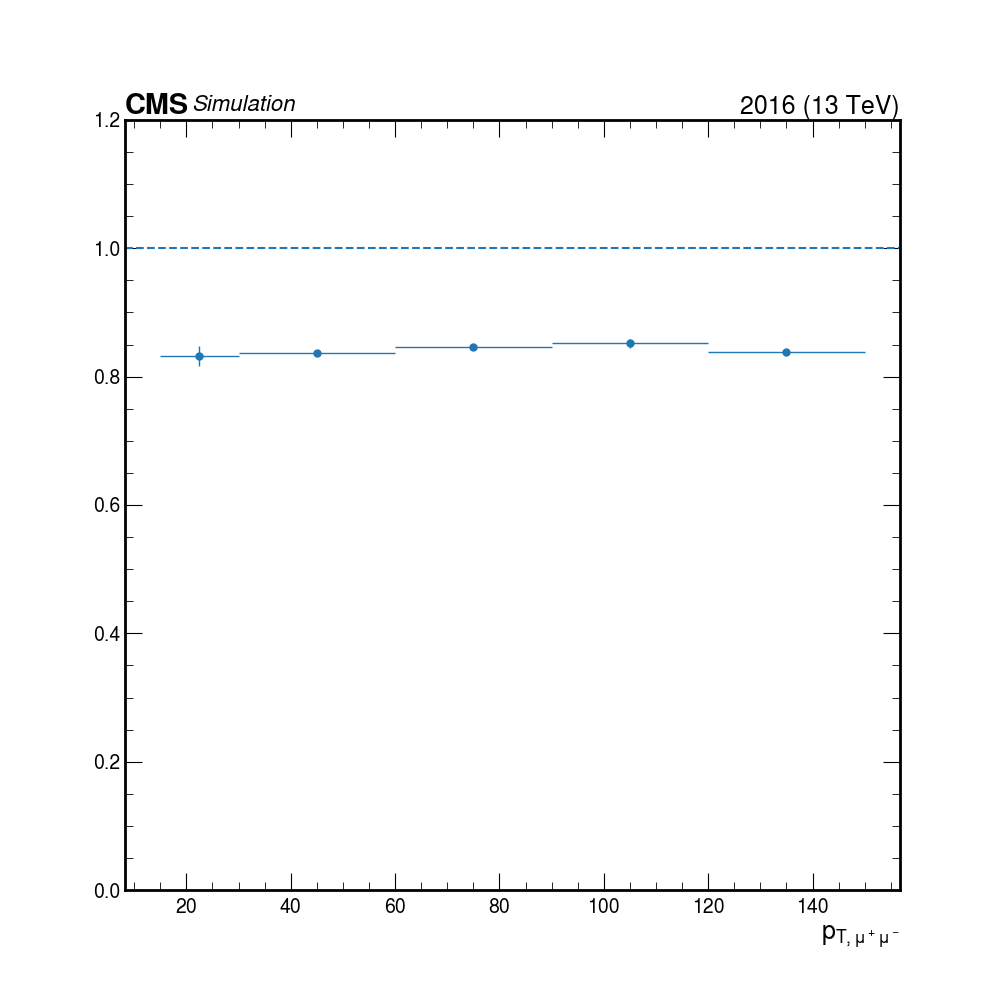
\includegraphics[width=0.44\textwidth]{figures/efficiency/acc_dimu_pt_2016.png}}}\hfill
  \subfloat[][]{\label{subfig:acc_dimu_rap_2016}%
    \fbox{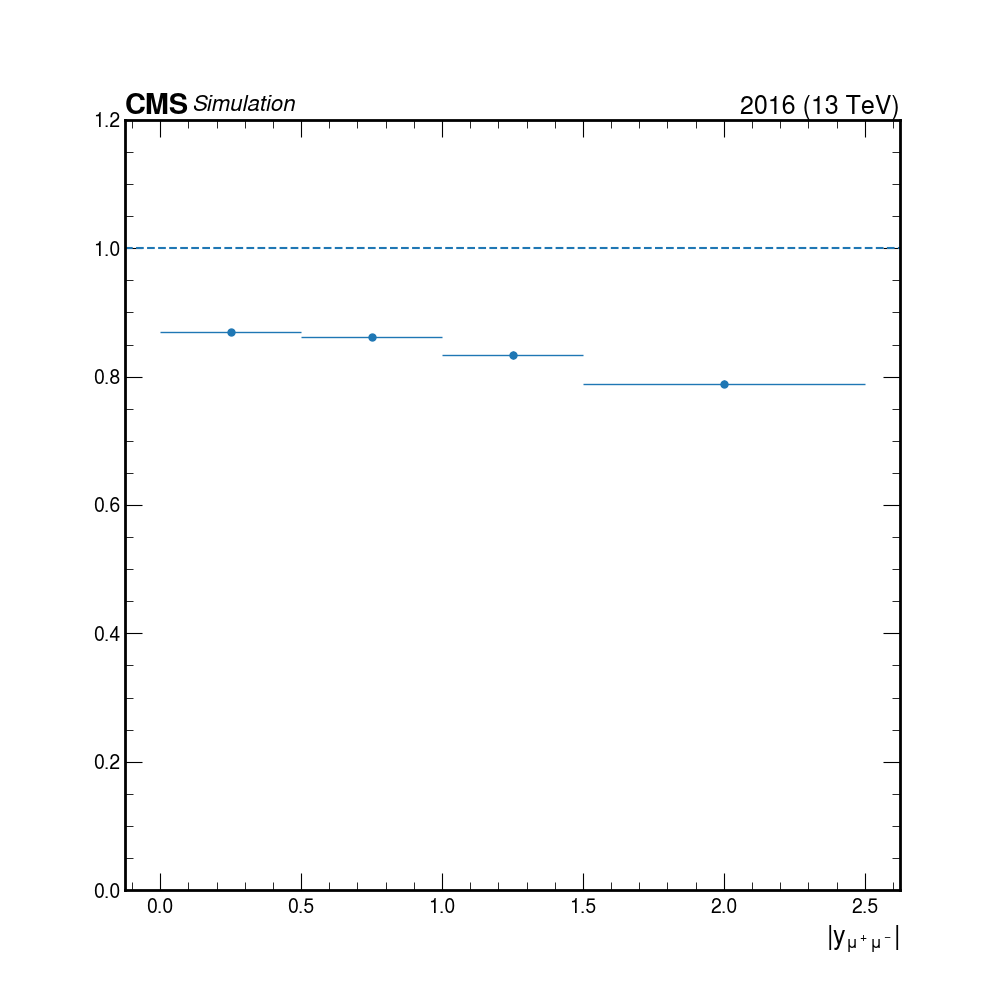
\includegraphics[width=0.44\textwidth]{figures/efficiency/acc_dimu_rap_2016.png}}}\hfill\\
  \subfloat[][]{\label{subfig:acc_dimu_2D_2016}%
    \fbox{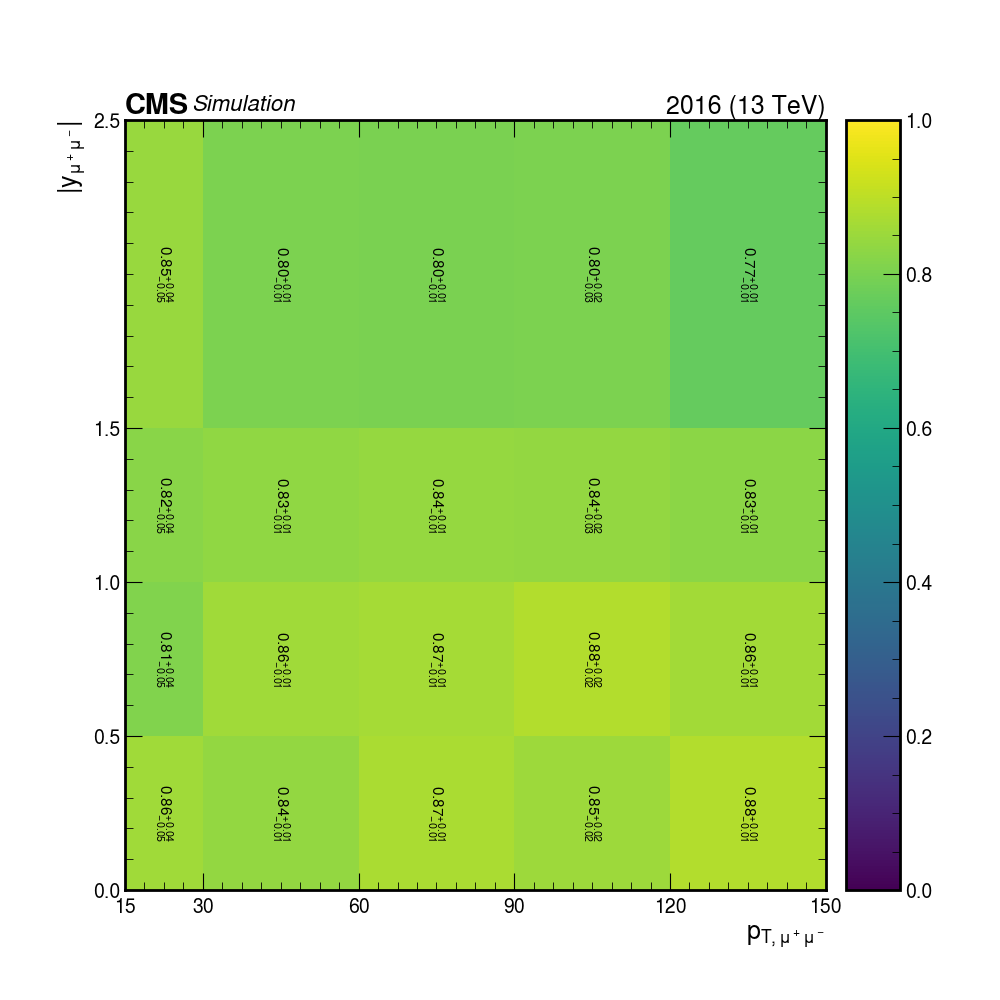
\includegraphics[width=0.44\textwidth]{figures/efficiency/acc_dimu_2016.png}}}\\
  \legend{$\Upsilon$ acceptance extracted from the 2016 MC data sample. The acceptance is given with respect to the dimuon $p_T$ in (a), $y$ in (b), and in both $p_T$ and $y$ in (c). In (a) and (b). The horizontal dashed line is set to the upper limit of the acceptance, one.}
\end{figure}

\begin{figure}[H]{15cm}
  \caption{D$^*$ acceptance of the selected associated $\Upsilon +$ D$^*$ extracted from 2016 MC sample.}
  \label{fig:acc_dstar_2016}
  \subfloat[][]{\label{subfig:acc_dstar_pt_2016}%
    \fbox{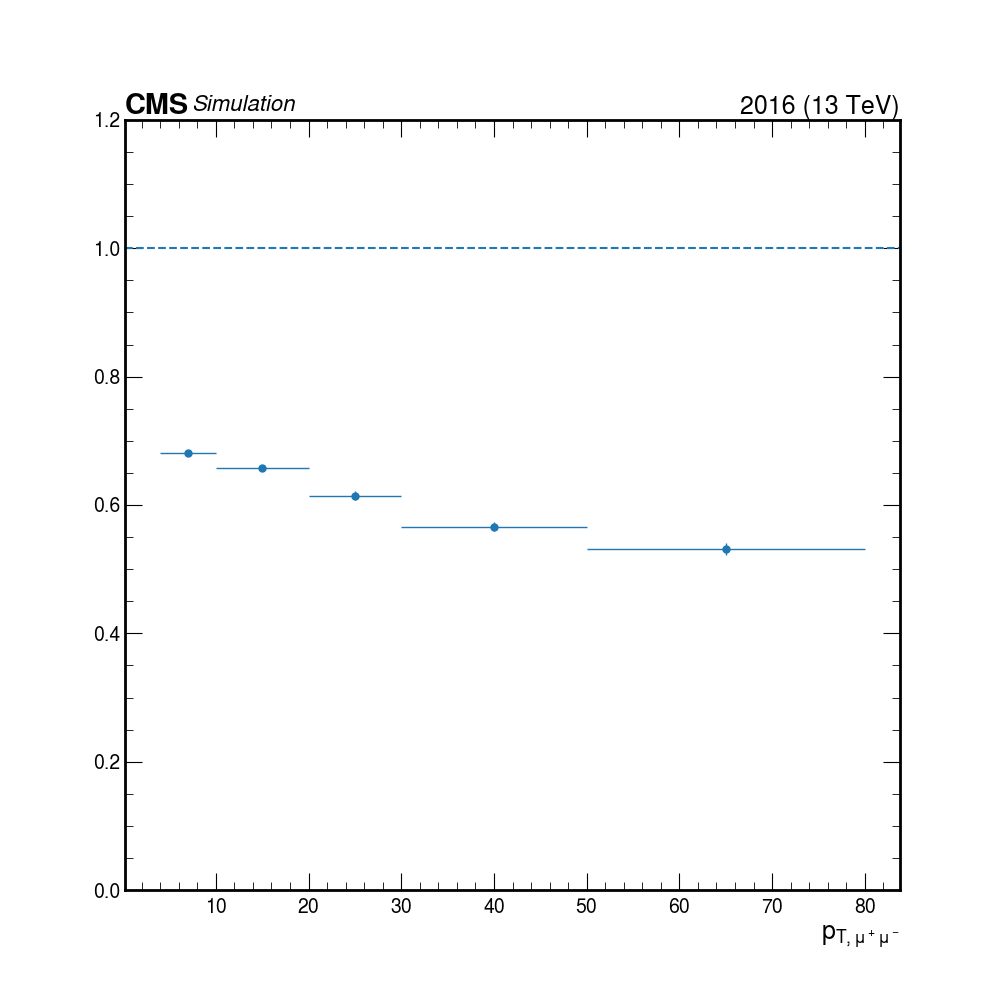
\includegraphics[width=0.44\textwidth]{figures/efficiency/acc_dstar_pt_2016.png}}}\hfill
  \subfloat[][]{\label{subfig:acc_dstar_rap_2016}%
    \fbox{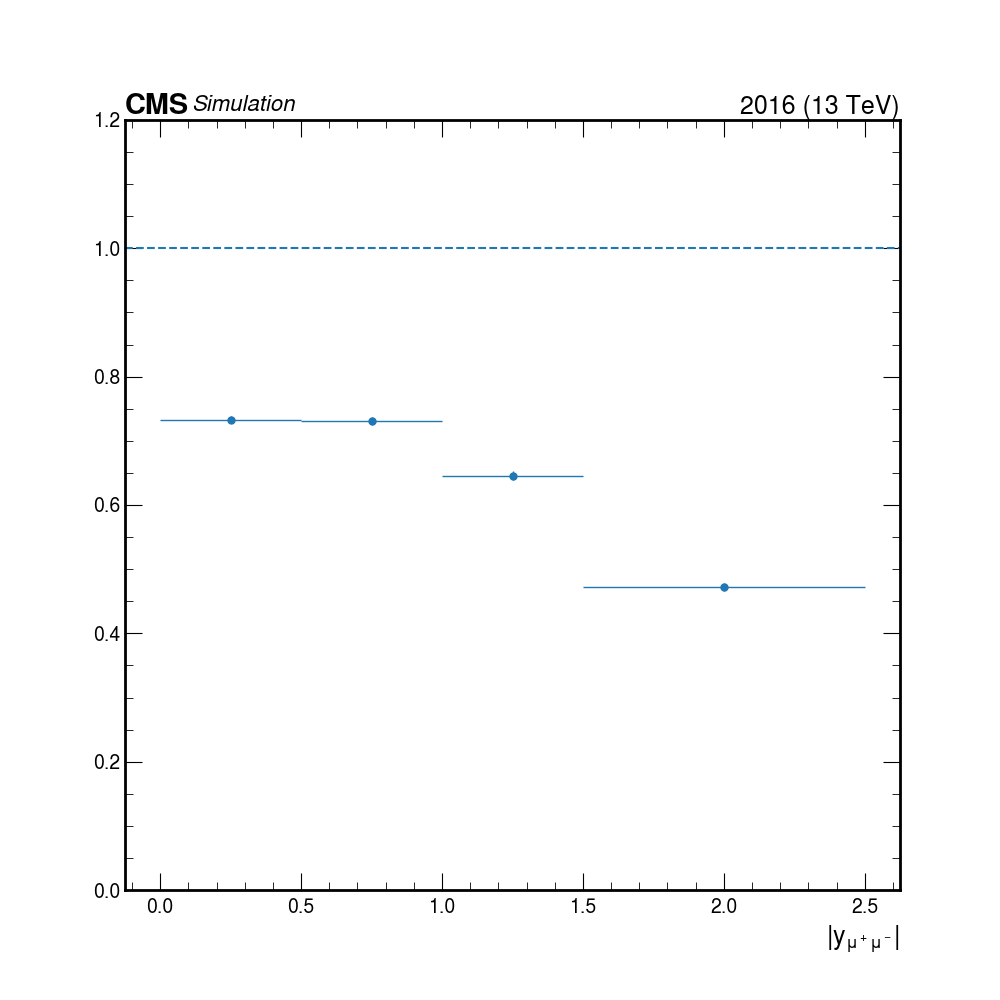
\includegraphics[width=0.44\textwidth]{figures/efficiency/acc_dstar_rap_2016.png}}}\hfill\\
  \subfloat[][]{\label{subfig:acc_dstar_2D_2016}%
    \fbox{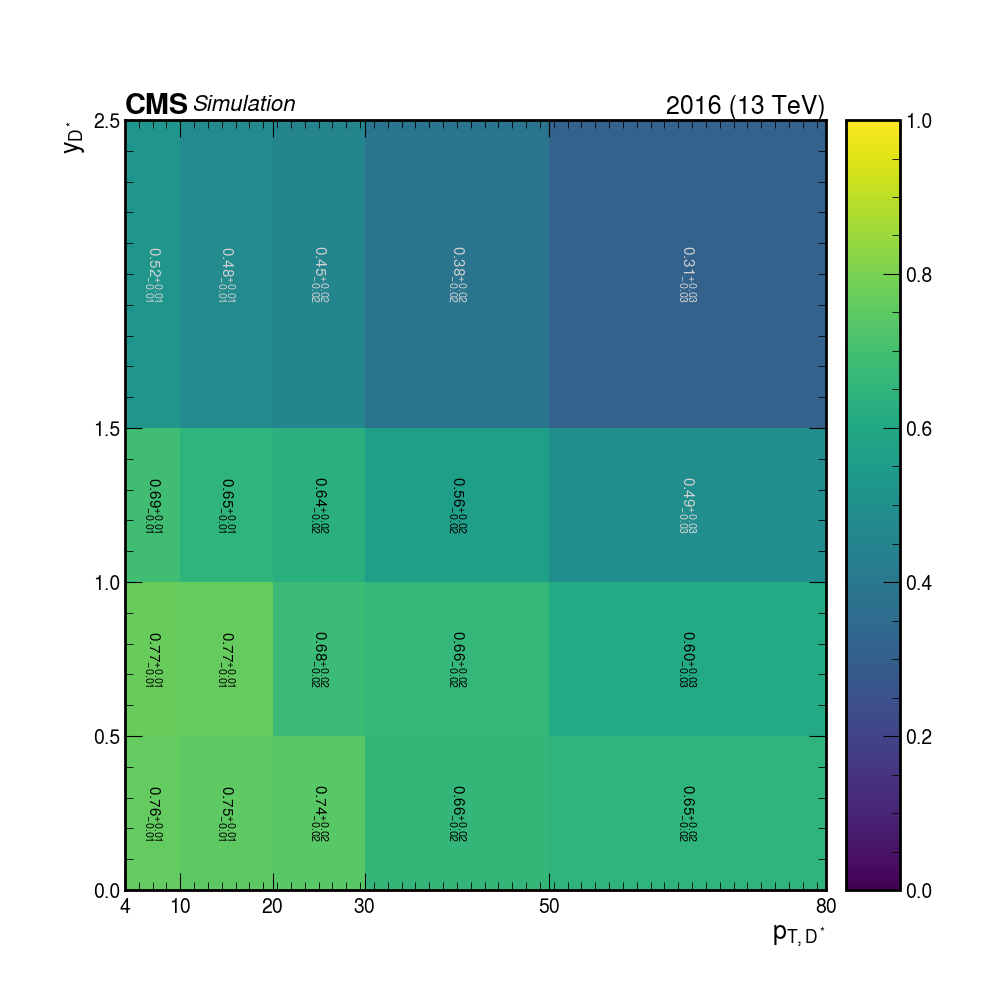
\includegraphics[width=0.44\textwidth]{figures/efficiency/acc_dstar_2016.png}}}\\
  \legend{D$^*$ acceptance extracted from the 2016 MC data sample. The acceptance is given with respect to the reconstructed D$^*$ $p_T$ in (a), $y$ in (b), and in both $p_T$ and $y$ in (c). In (a) and (b). The horizontal dashed line is set to the upper limit of the acceptance, one.}
\end{figure}

\begin{figure}[H]{15cm}
  \caption{$\Upsilon$ selection cuts efficiency of the selected associated $\Upsilon +$ D$^*$ extracted from 2016 MC sample.}
  \label{fig:eff_cuts_dimu_2016}
  \subfloat[][]{\label{subfig:eff_cuts_dimu_pt_2016}%
  \fbox{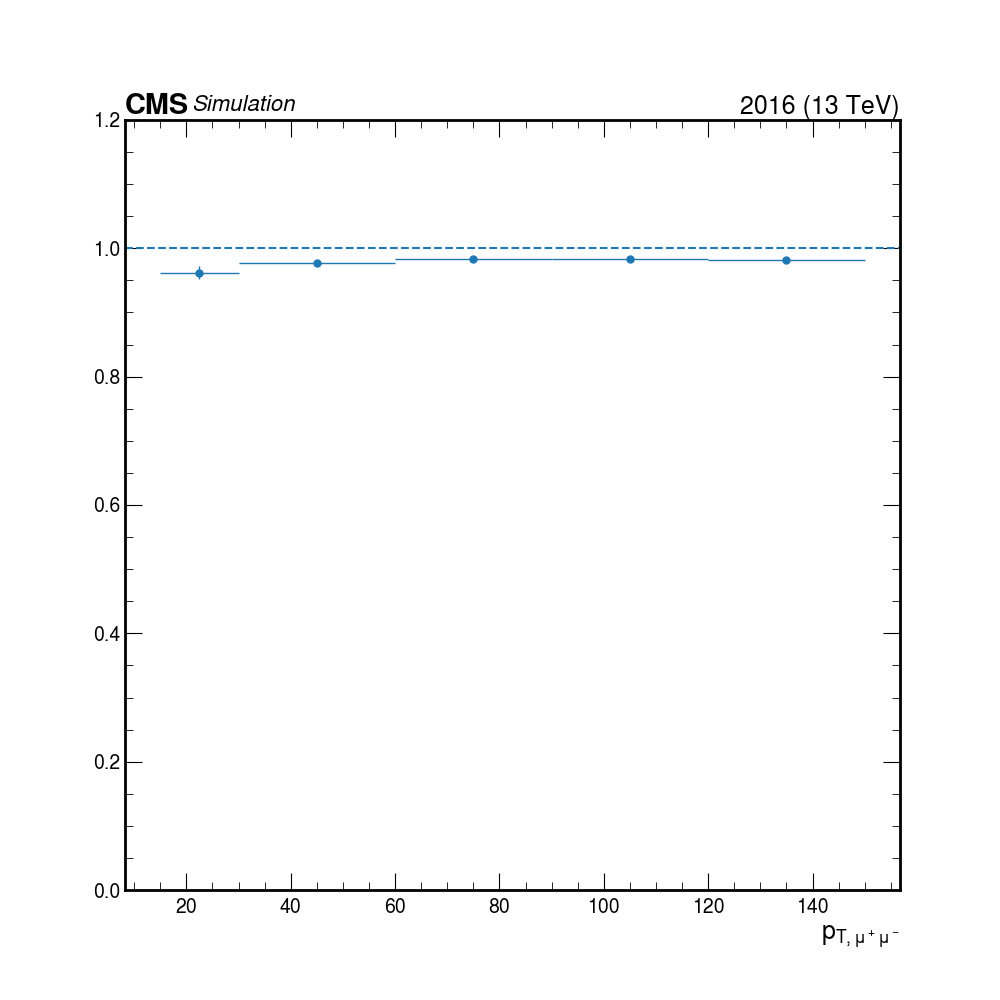
\includegraphics[width=0.44\textwidth]{figures/efficiency/eff_cuts_dimu_pt_2016.png}}}\hfill
  \subfloat[][]{\label{subfig:eff_cuts_dimu_rap_2016}%
  \fbox{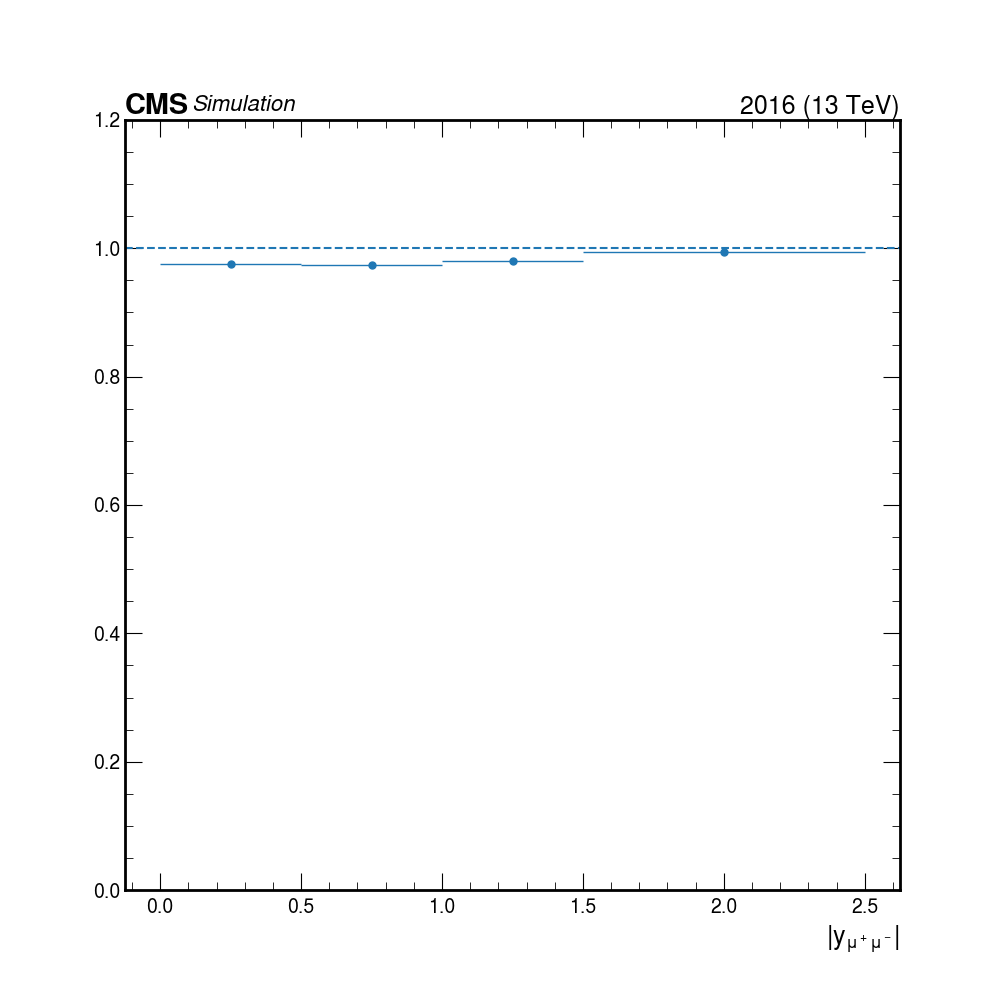
\includegraphics[width=0.44\textwidth]{figures/efficiency/eff_cuts_dimu_rap_2016.png}}}\hfill\\
  \subfloat[][]{\label{subfig:eff_cuts_dimu_2D_2016}%
  \fbox{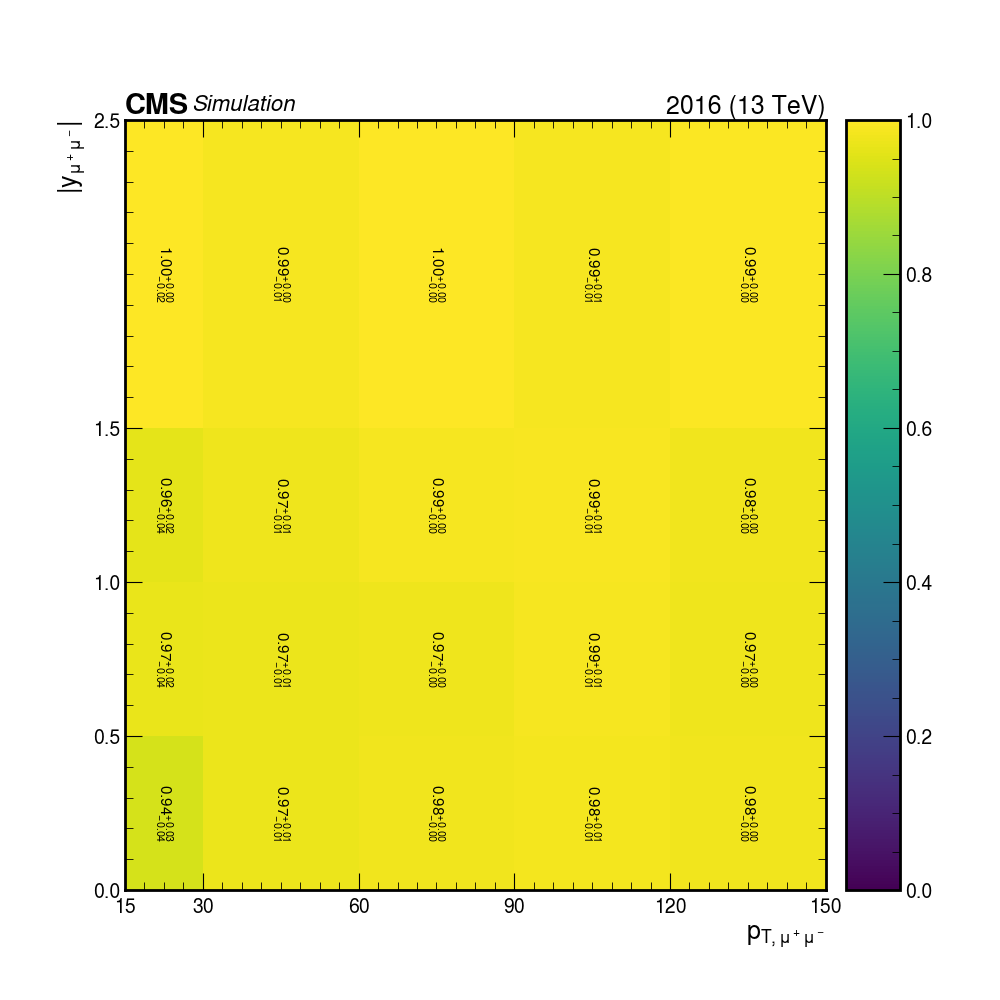
\includegraphics[width=0.44\textwidth]{figures/efficiency/eff_cuts_dimu_2016.png}}}\\
  \legend{$\Upsilon$ selection cuts efficiency extracted from the 2016 MC data sample. This efficiency is given with respect to the dimuon $p_T$ in (a), $y$ in (b), and in both $p_T$ and $y$ in (c). In (a) and (b). The horizontal dashed line is set to the upper limit of the efficiency.}
\end{figure}

\begin{figure}[H]{15cm}
  \caption{D$^*$ selection cuts efficiency of the selected associated $\Upsilon +$ D$^*$ extracted from 2016 MC sample.}
  \label{fig:eff_cuts_dstar_2016}
  \subfloat[][]{\label{subfig:eff_cuts_dstar_pt_2016}%
    \fbox{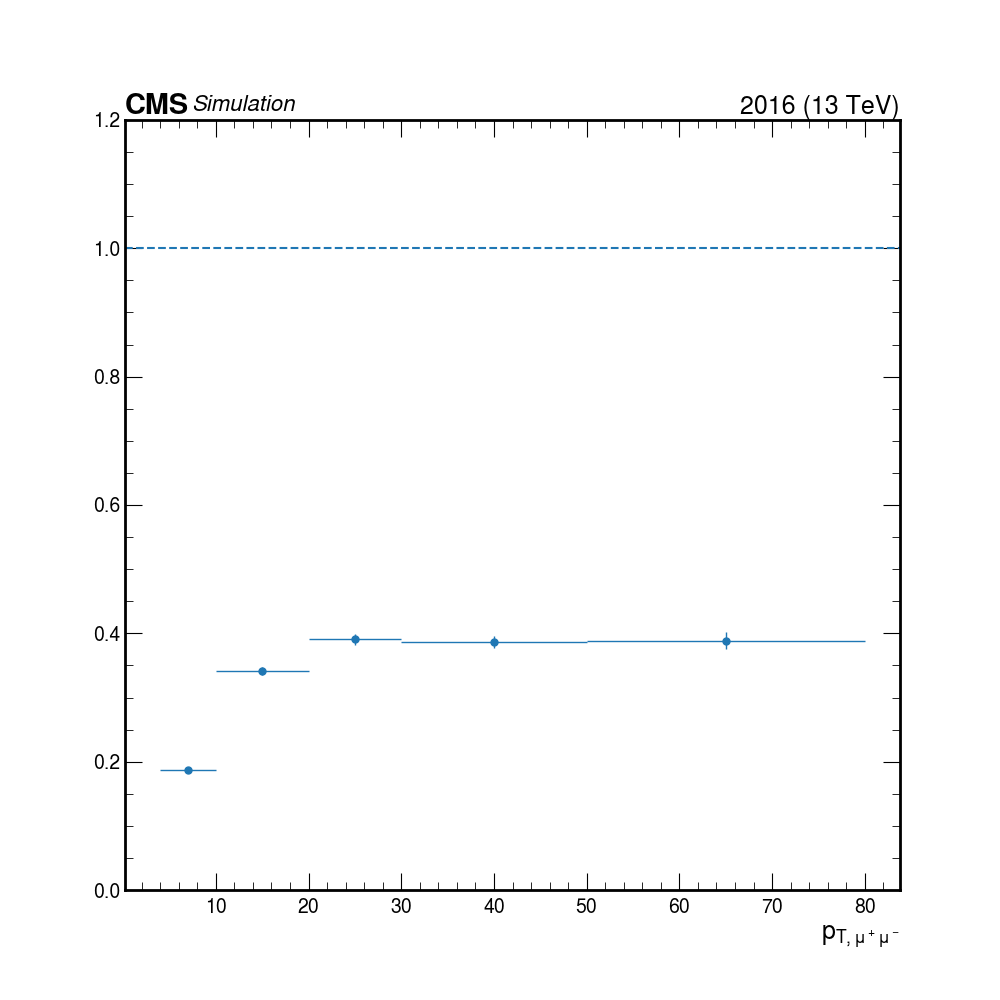
\includegraphics[width=0.44\textwidth]{figures/efficiency/eff_cuts_dstar_pt_2016.png}}}\hfill
  \subfloat[][]{\label{subfig:eff_cuts_dstar_rap_2016}%
    \fbox{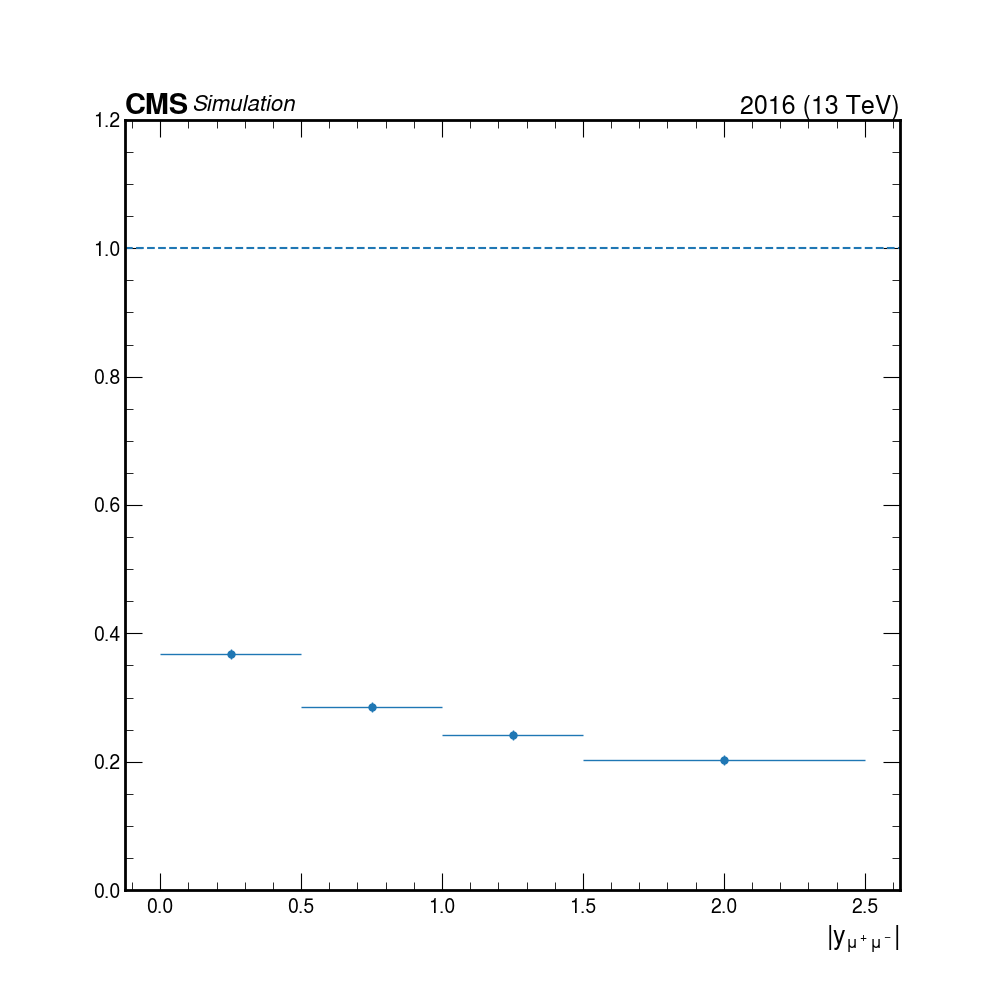
\includegraphics[width=0.44\textwidth]{figures/efficiency/eff_cuts_dstar_rap_2016.png}}}\hfill\\
  \subfloat[][]{\label{subfig:eff_cuts_dstar_2D_2016}%
    \fbox{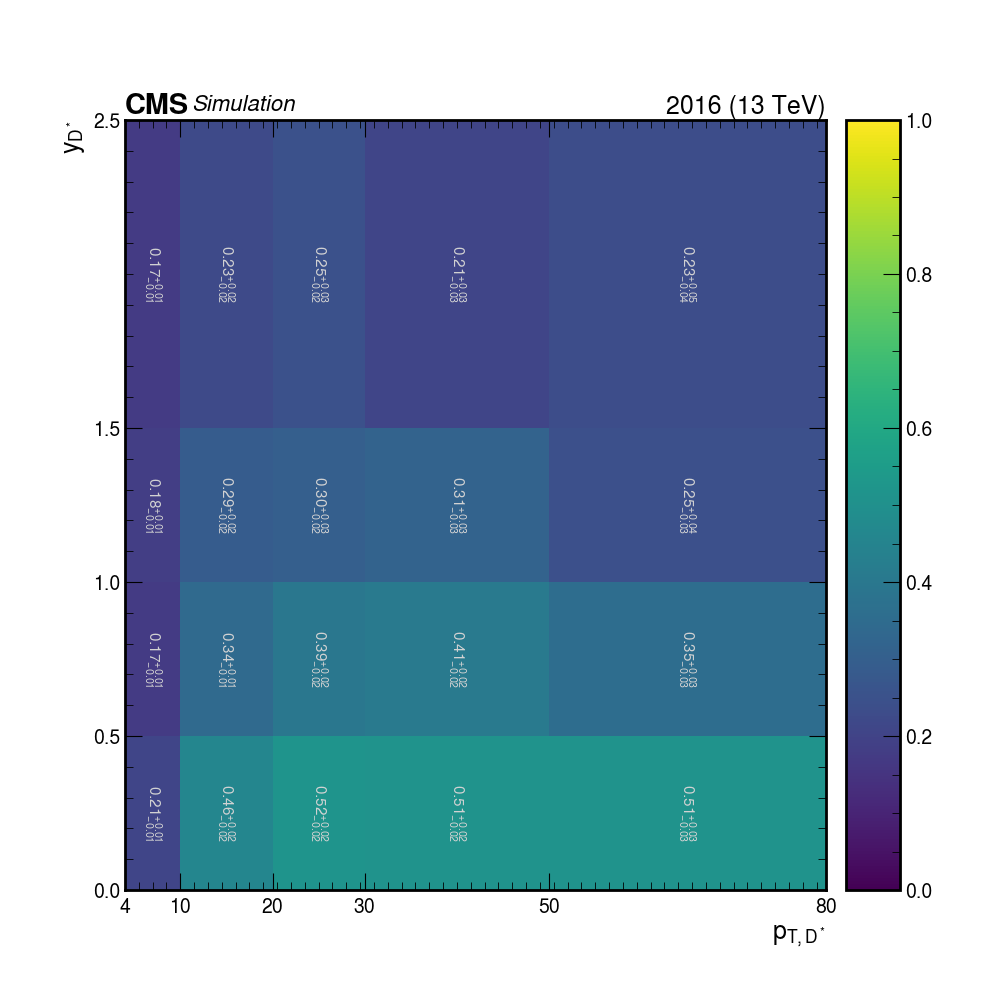
\includegraphics[width=0.44\textwidth]{figures/efficiency/eff_cuts_dstar_2016.png}}}\\
  \legend{D$^*$ selection cuts efficiency extracted from the 2016 MC data sample. This efficiency is given with respect to the D$^*$ $p_T$ in (a), $y$ in (b), and in both $p_T$ and $y$ in (c). In (a) and (b). The horizontal dashed line is set to the upper limit of the efficiency.}
\end{figure}

\begin{figure}[H]{15cm}
  \caption{Trigger efficiency of the selected associated $\Upsilon +$ D$^*$ extracted from 2016 MC sample.}
  \label{fig:eff_trigger_2016}
  \subfloat[][]{\label{subfig:eff_trigger_pt_2016}%
    \fbox{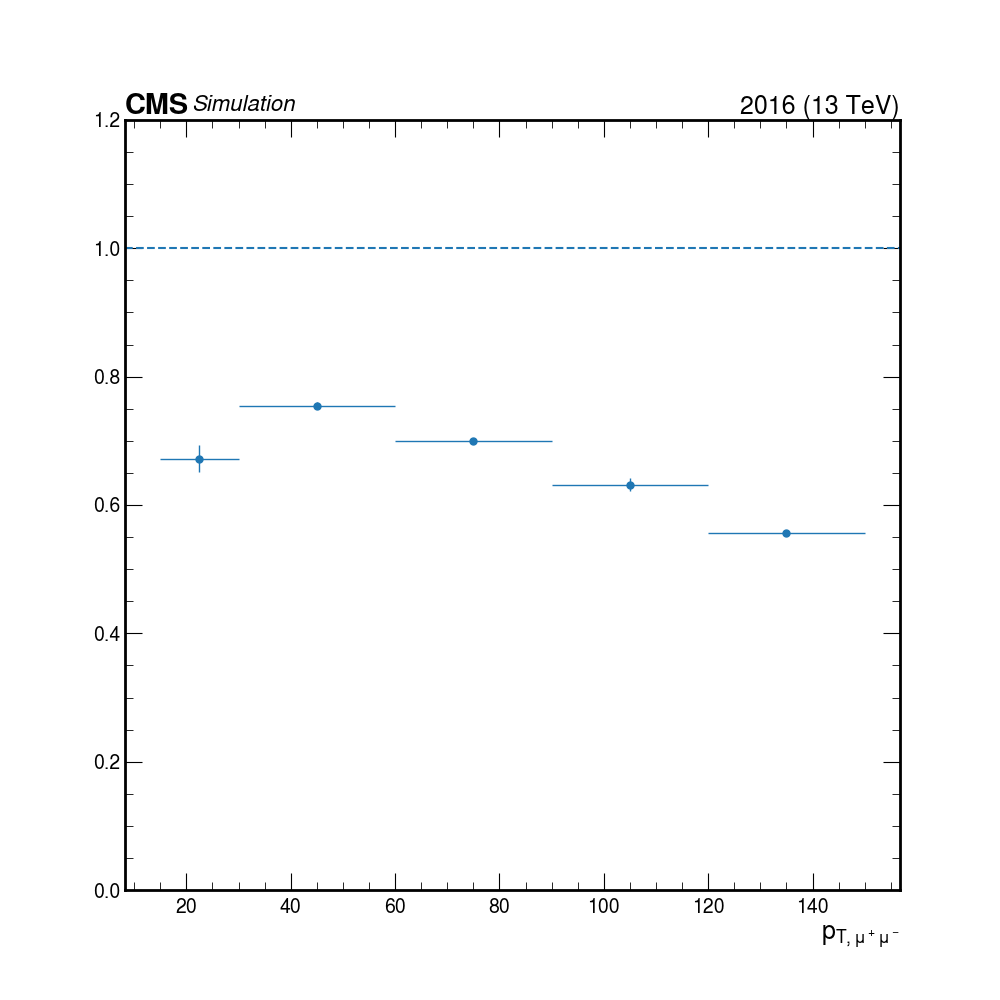
\includegraphics[width=0.44\textwidth]{figures/efficiency/eff_trigger_pt_2016.png}}}\hfill
  \subfloat[][]{\label{subfig:eff_trigger_rap_2016}%
    \fbox{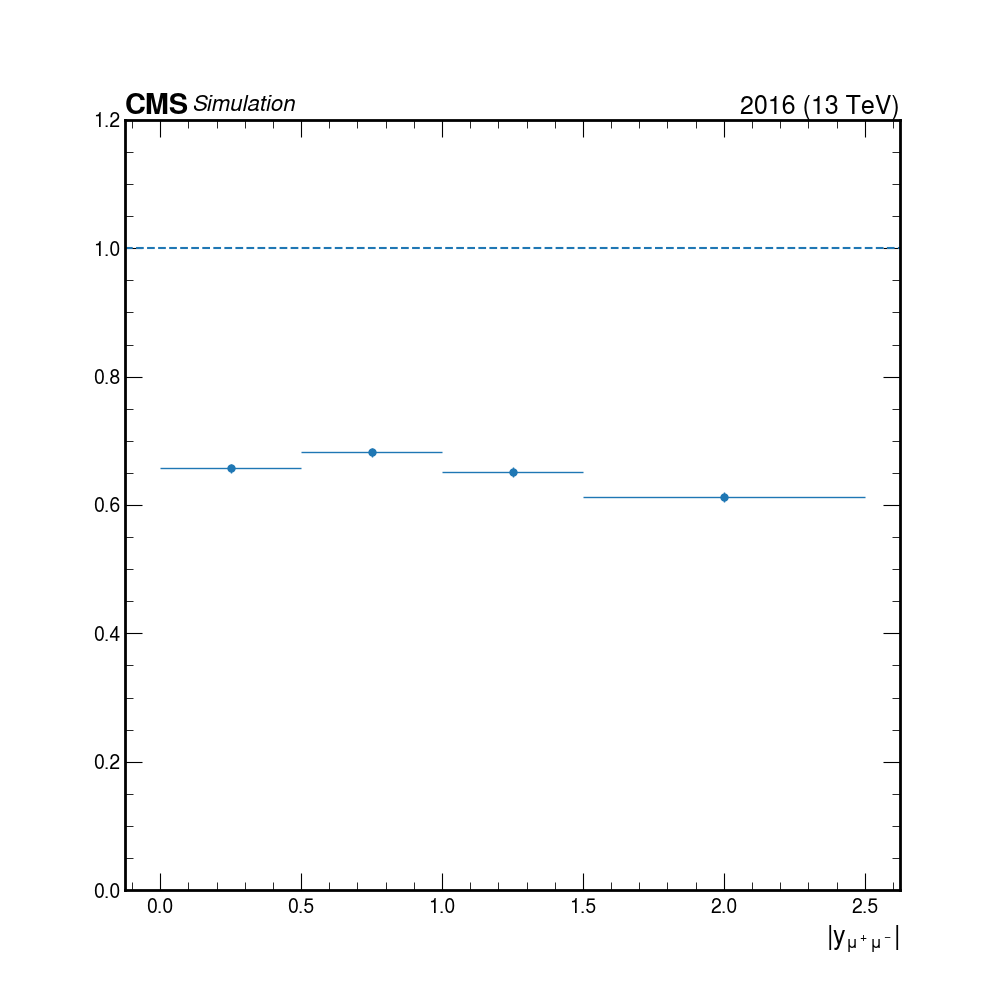
\includegraphics[width=0.44\textwidth]{figures/efficiency/eff_trigger_rap_2016.png}}}\hfill\\
  \subfloat[][]{\label{subfig:eff_trigger_2D_2016}%
    \fbox{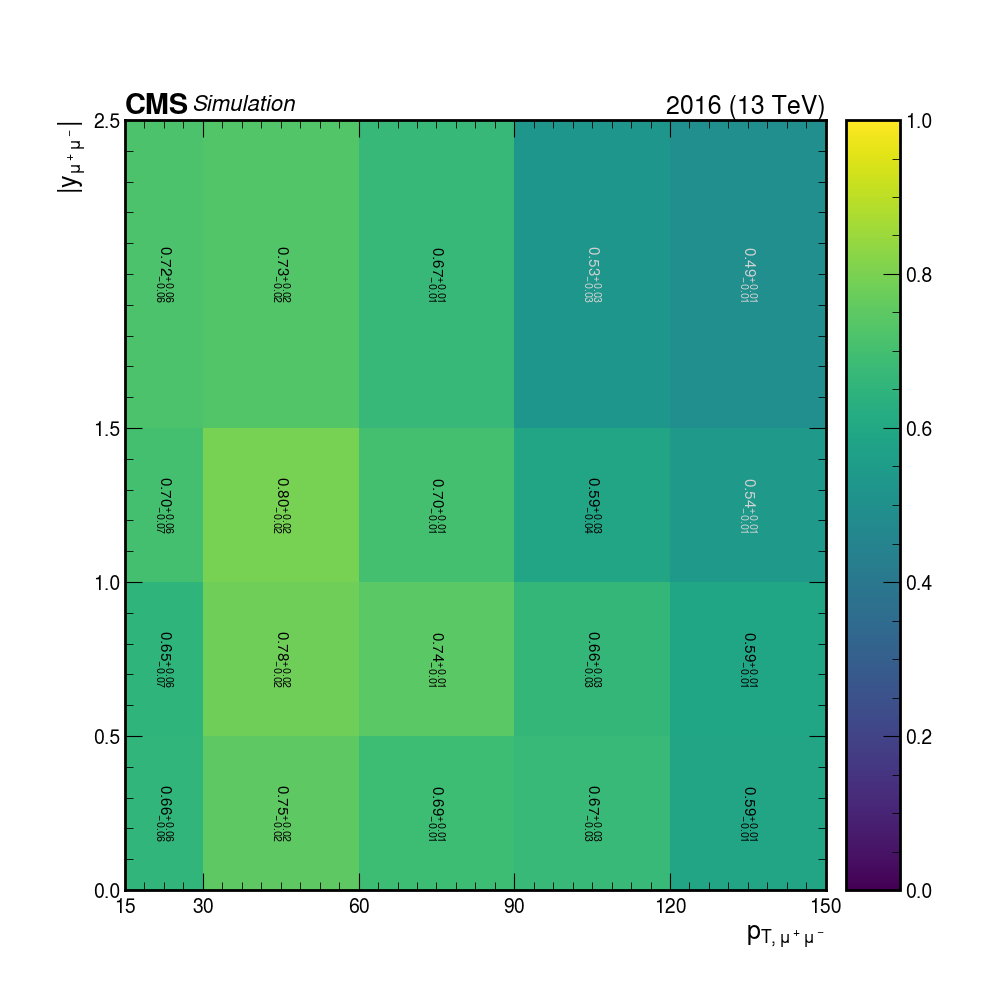
\includegraphics[width=0.44\textwidth]{figures/efficiency/eff_trigger_2016.png}}}\\
  \legend{Trigger efficiency extracted from the 2016 MC data sample. This efficiency is given with respect to the dimuon $p_T$ in (a), $y$ in (b), and in both $p_T$ and $y$ in (c). In (a) and (b). The horizontal dashed line is set to the upper limit of the efficiency.}
\end{figure}

\begin{figure}[H]{15cm}
  \caption{Trigger efficiency of the selected associated $\Upsilon +$ D$^*$ extracted from 2016 MC sample.}
  \label{fig:eff_asso_2016}
  \subfloat[][]{\label{subfig:eff_asso_pt_2016}%
    \fbox{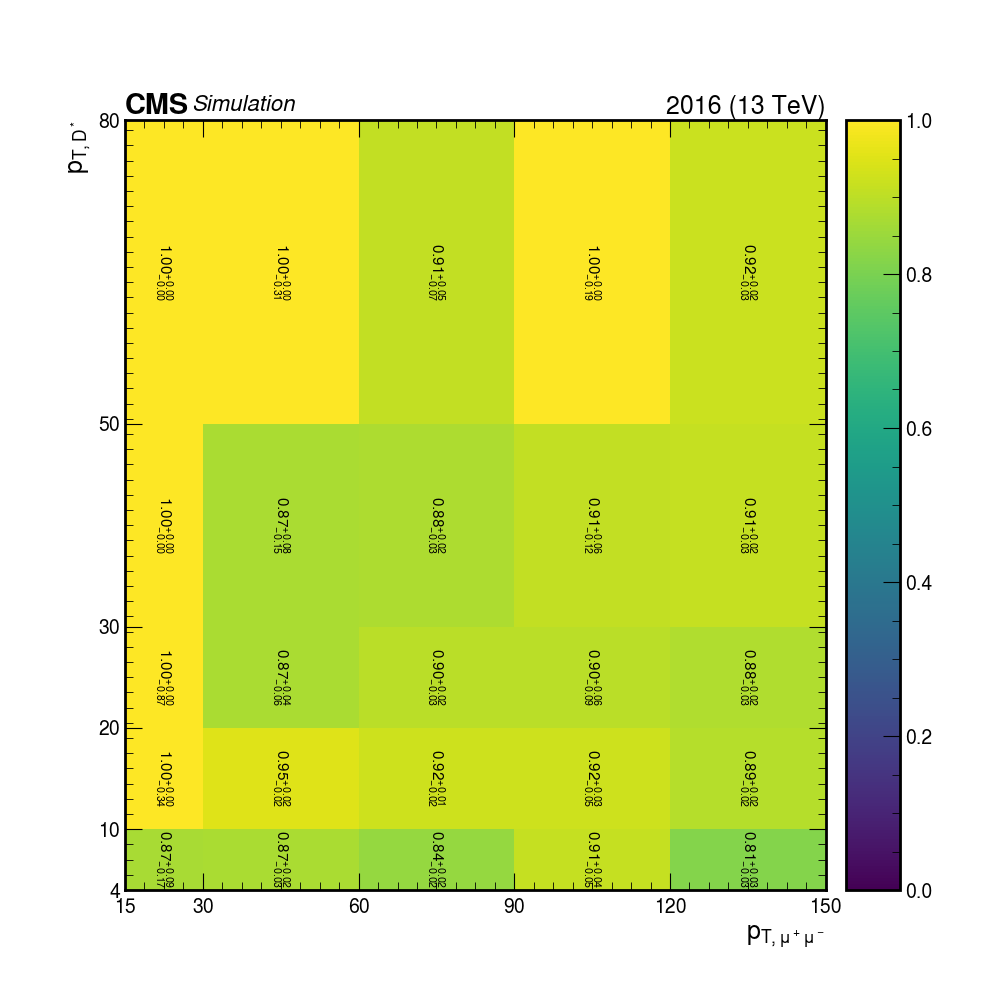
\includegraphics[width=0.44\textwidth]{figures/efficiency/eff_asso_pt_2016.png}}}\hfill
  \subfloat[][]{\label{subfig:eff_asso_rap_2016}%
    \fbox{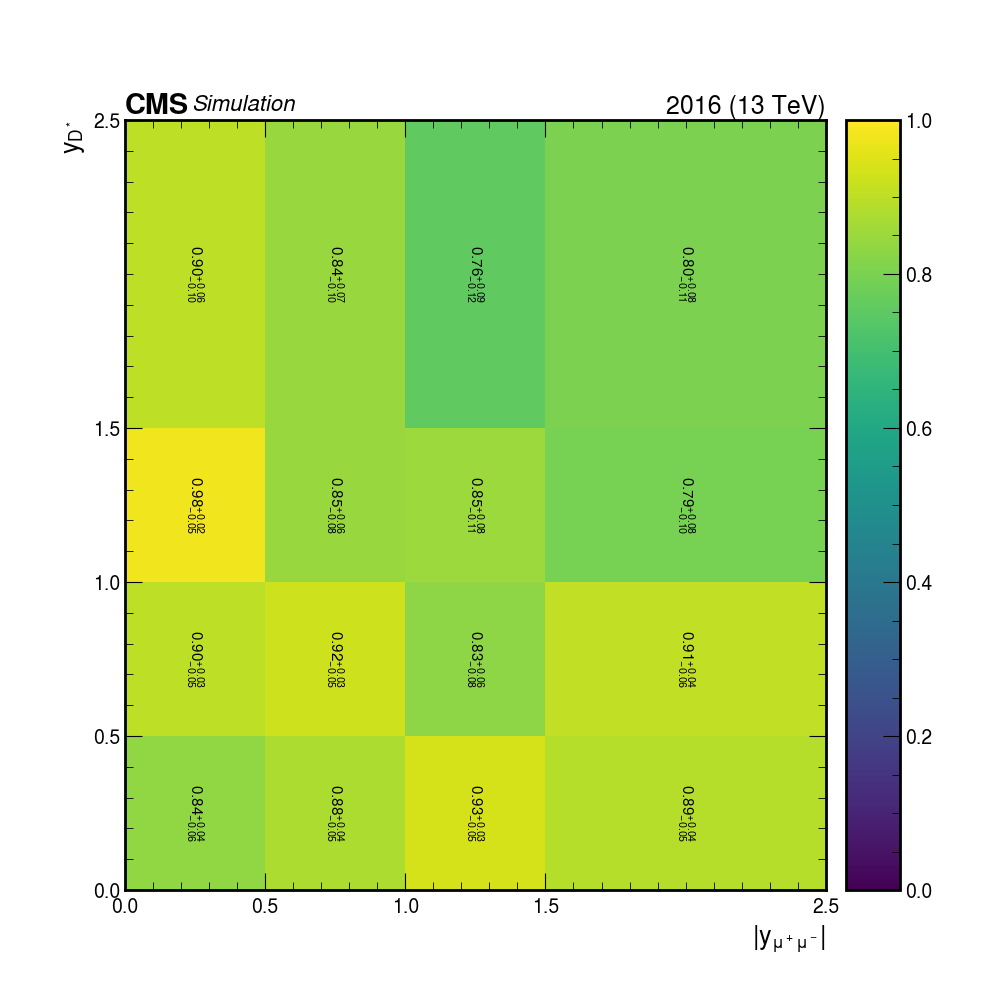
\includegraphics[width=0.44\textwidth]{figures/efficiency/eff_asso_rap_2016.png}}}\hfill\\
  \legend{Association efficiency extracted from the 2016 MC data sample. The efficiency maps are given with respect to the dimuon and D$^*$ $p_T$ in (a) and $y$ in (b).}
\end{figure}

\clearpage

\section{Efficiencies for sample 2017}

\begin{figure}[H]{15cm}
  \caption{$\Upsilon$ acceptance of the selected associated $\Upsilon +$ D$^*$ extracted from 2017 MC sample.}
  \label{fig:acc_dimu_2017}
  \subfloat[][]{\label{subfig:acc_dimu_pt_2017}%
    \fbox{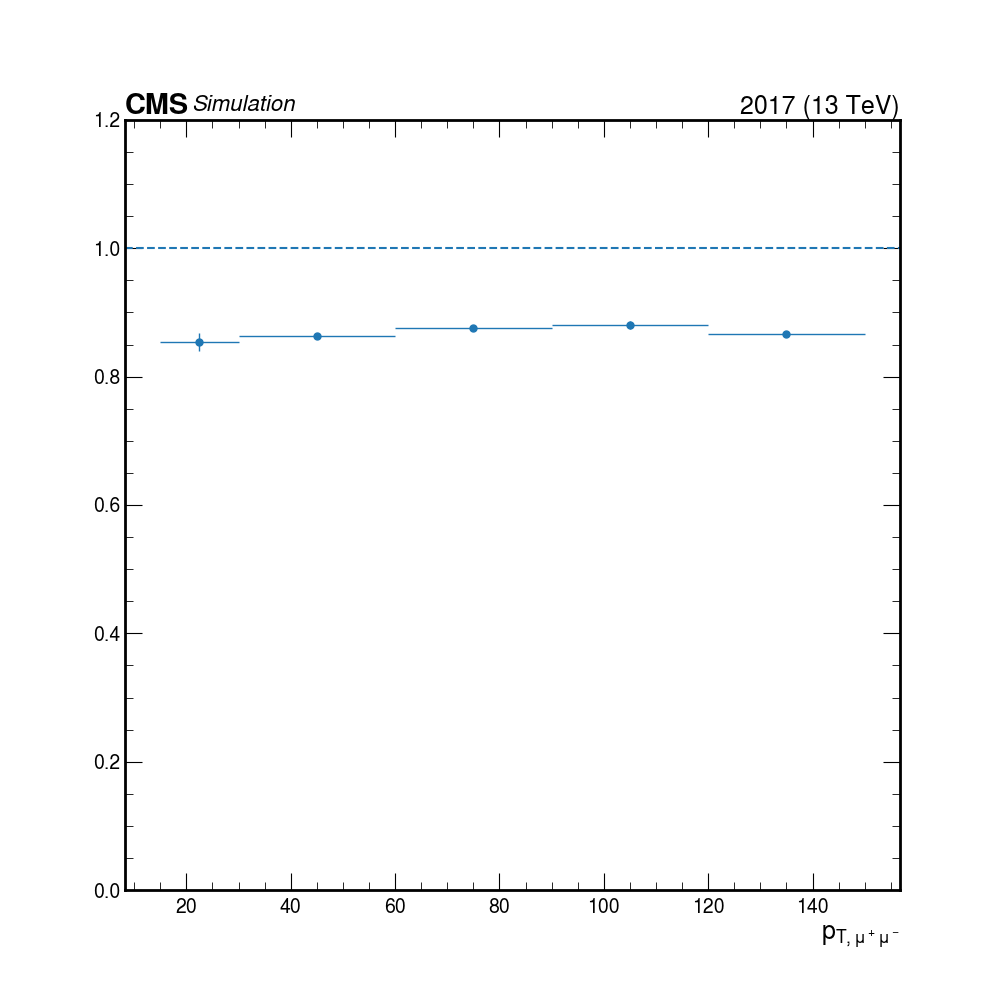
\includegraphics[width=0.44\textwidth]{figures/efficiency/acc_dimu_pt_2017.png}}}\hfill
  \subfloat[][]{\label{subfig:acc_dimu_rap_2017}%
    \fbox{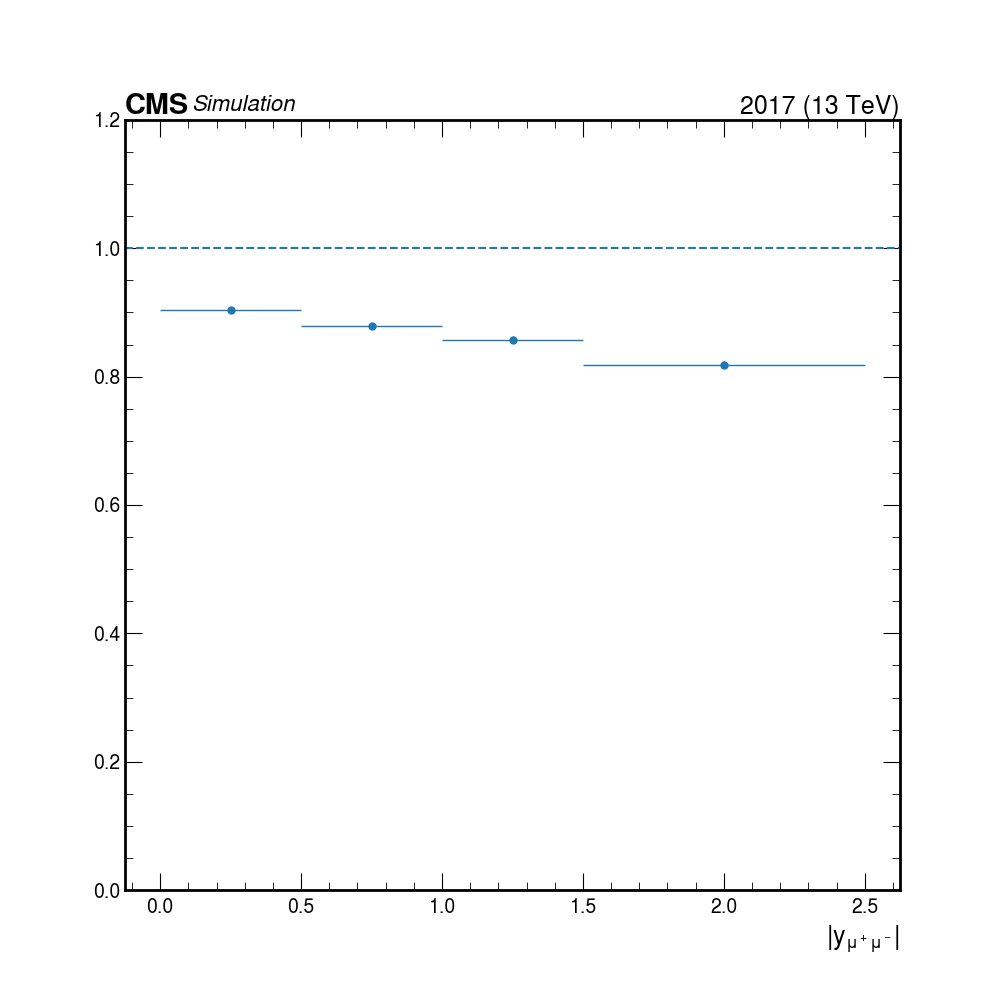
\includegraphics[width=0.44\textwidth]{figures/efficiency/acc_dimu_rap_2017.png}}}\hfill\\
  \subfloat[][]{\label{subfig:acc_dimu_2D_2017}%
    \fbox{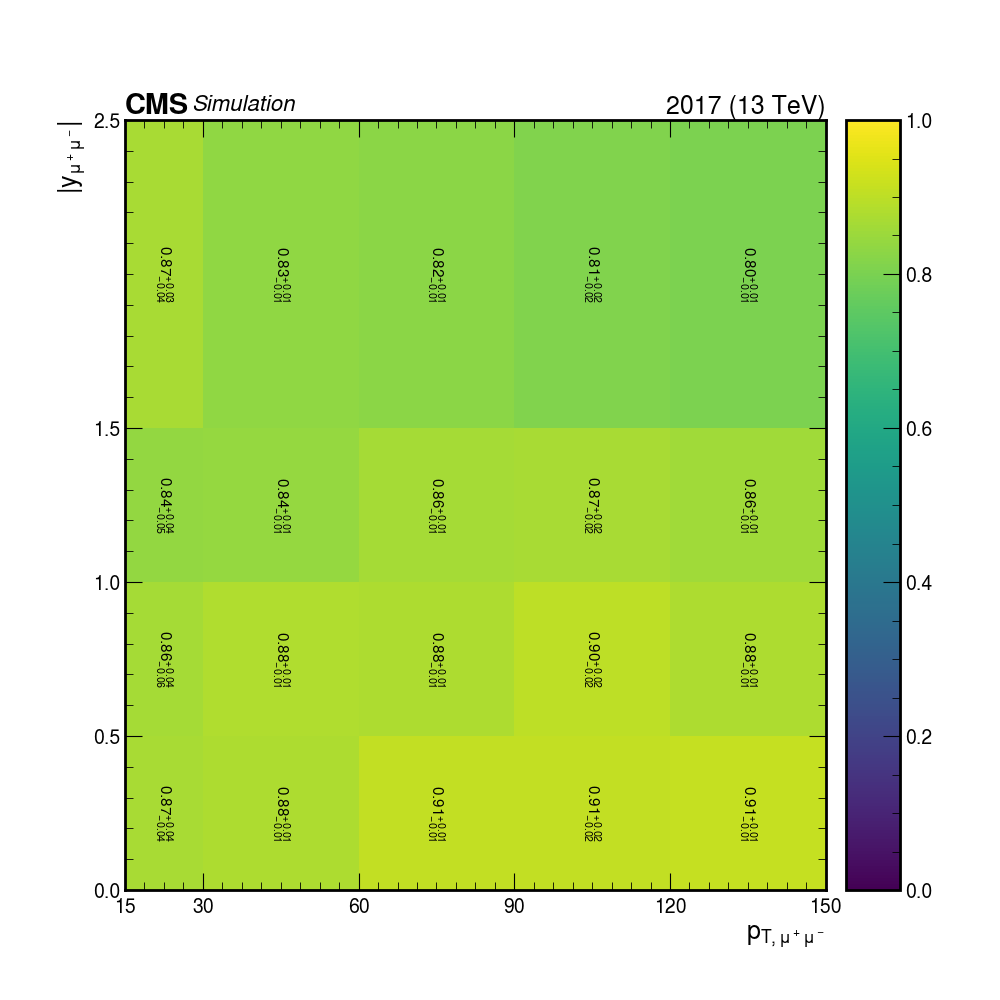
\includegraphics[width=0.44\textwidth]{figures/efficiency/acc_dimu_2017.png}}}\\
  \legend{$\Upsilon$ acceptance extracted from the 2017 MC data sample. The acceptance is given with respect to the dimuon $p_T$ in (a), $y$ in (b), and in both $p_T$ and $y$ in (c). In (a) and (b). The horizontal dashed line is set to the upper limit of the acceptance, one.}
\end{figure}

\begin{figure}[H]{15cm}
  \caption{D$^*$ acceptance of the selected associated $\Upsilon +$ D$^*$ extracted from 2017 MC sample.}
  \label{fig:acc_dstar_2017}
  \subfloat[][]{\label{subfig:acc_dstar_pt_2017}%
    \fbox{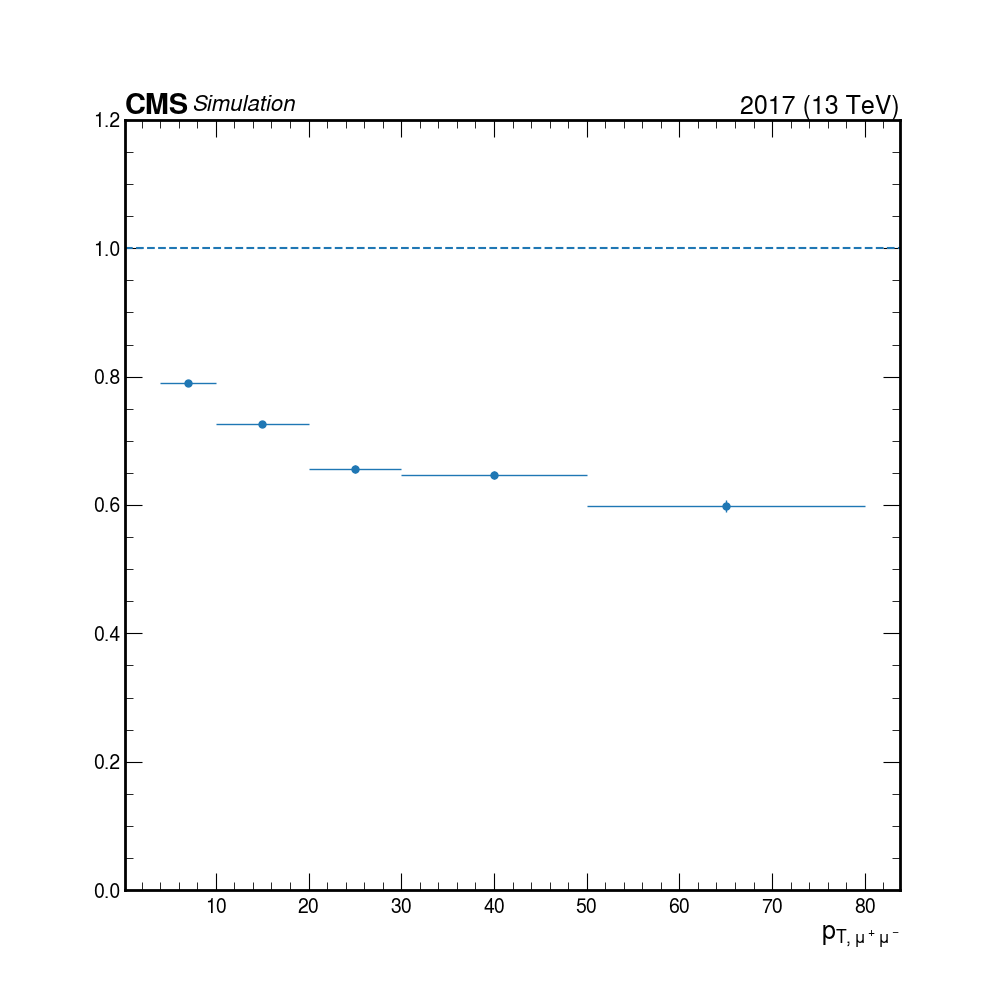
\includegraphics[width=0.44\textwidth]{figures/efficiency/acc_dstar_pt_2017.png}}}\hfill
  \subfloat[][]{\label{subfig:acc_dstar_rap_2017}%
    \fbox{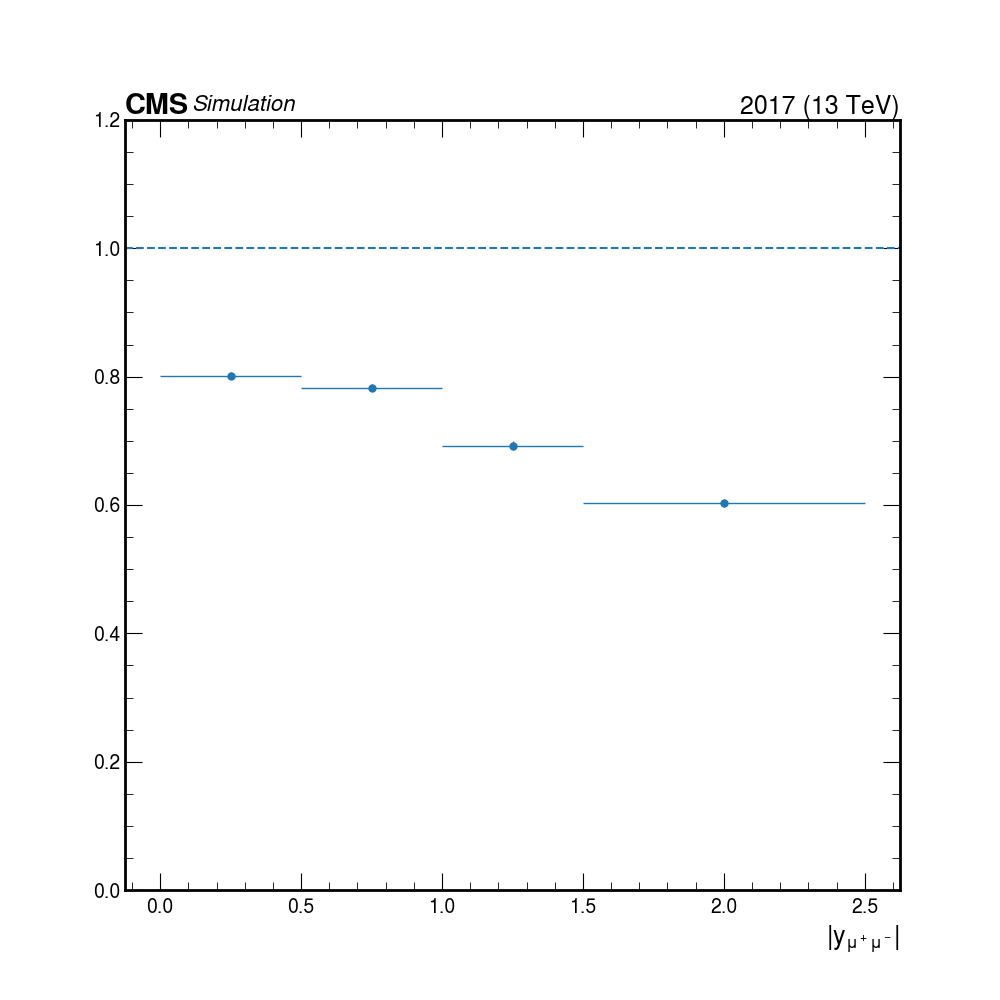
\includegraphics[width=0.44\textwidth]{figures/efficiency/acc_dstar_rap_2017.png}}}\hfill\\
  \subfloat[][]{\label{subfig:acc_dstar_2D_2017}%
    \fbox{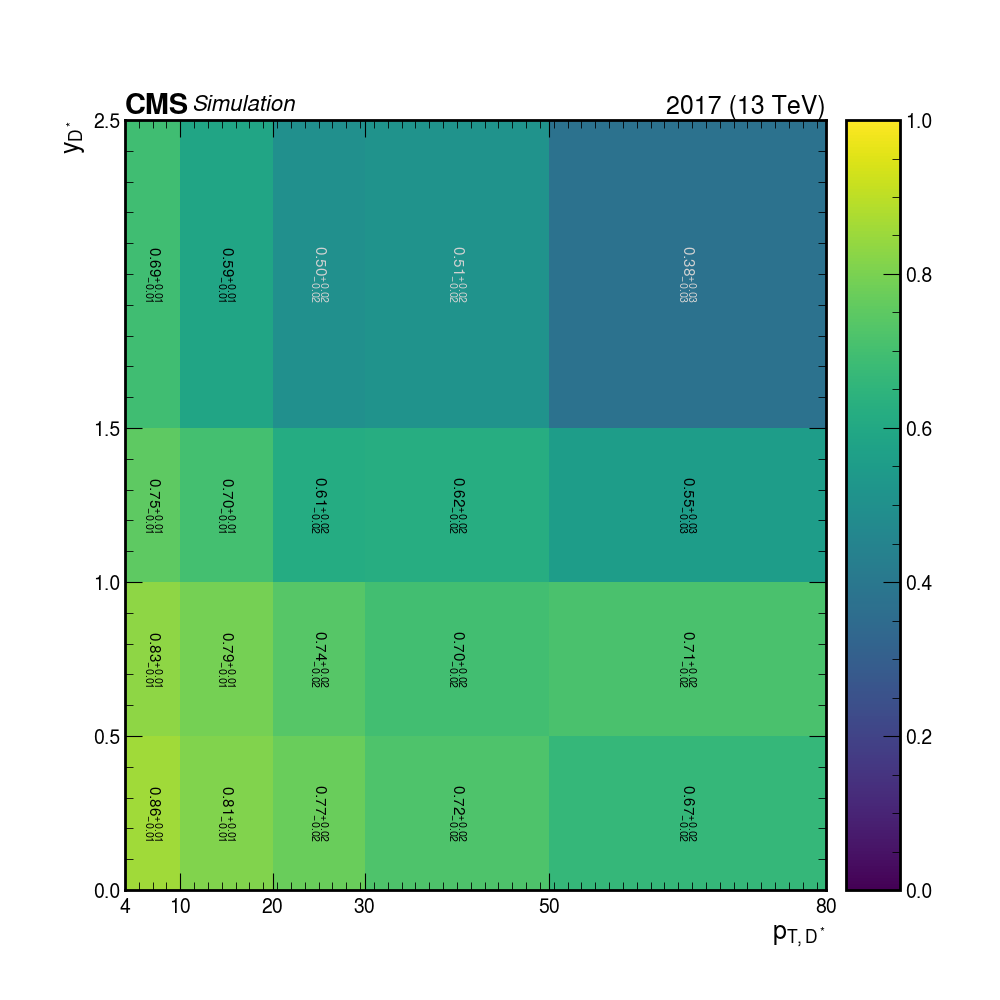
\includegraphics[width=0.44\textwidth]{figures/efficiency/acc_dstar_2017.png}}}\\
  \legend{D$^*$ acceptance extracted from the 2017 MC data sample. The acceptance is given with respect to the reconstructed D$^*$ $p_T$ in (a), $y$ in (b), and in both $p_T$ and $y$ in (c). In (a) and (b). The horizontal dashed line is set to the upper limit of the acceptance, one.}
\end{figure}

\begin{figure}[H]{15cm}
  \caption{$\Upsilon$ selection cuts efficiency of the selected associated $\Upsilon +$ D$^*$ extracted from 2017 MC sample.}
  \label{fig:eff_cuts_dimu_2017}
  \subfloat[][]{\label{subfig:eff_cuts_dimu_pt_2017}%
  \fbox{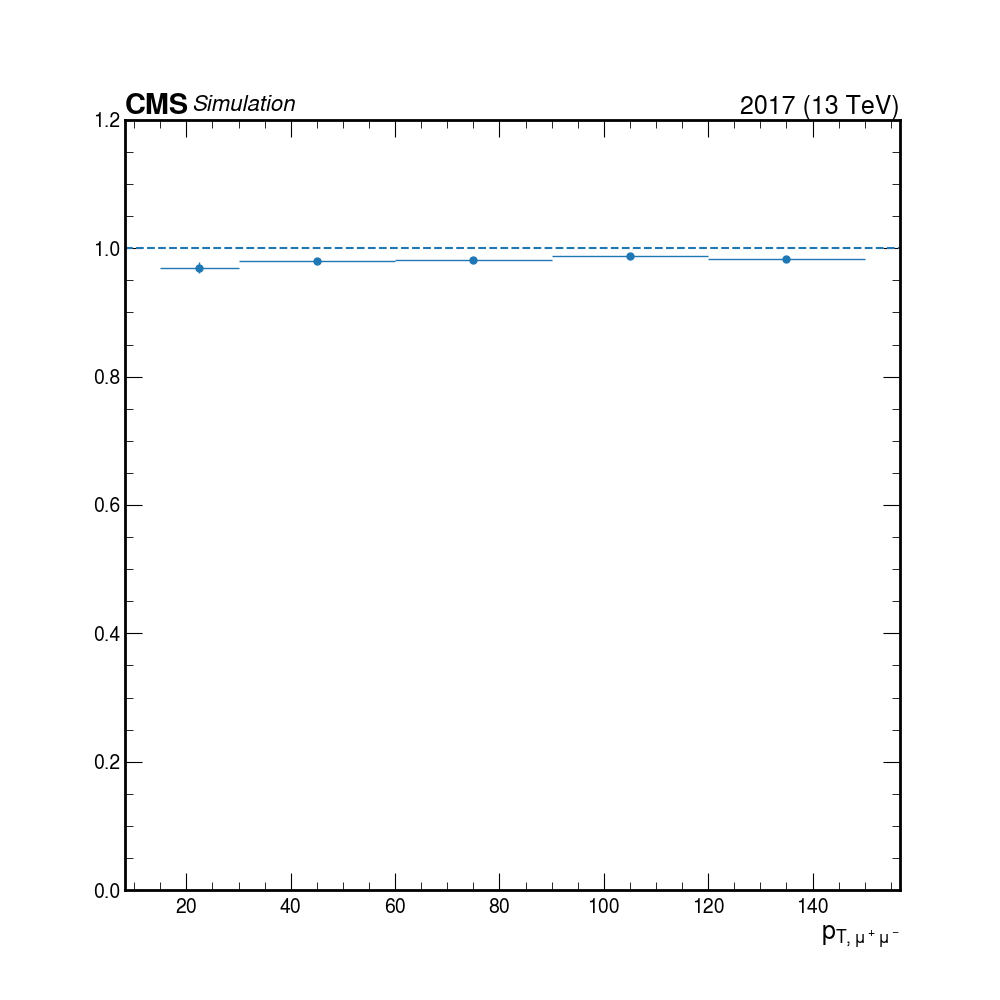
\includegraphics[width=0.44\textwidth]{figures/efficiency/eff_cuts_dimu_pt_2017.png}}}\hfill
  \subfloat[][]{\label{subfig:eff_cuts_dimu_rap_2017}%
  \fbox{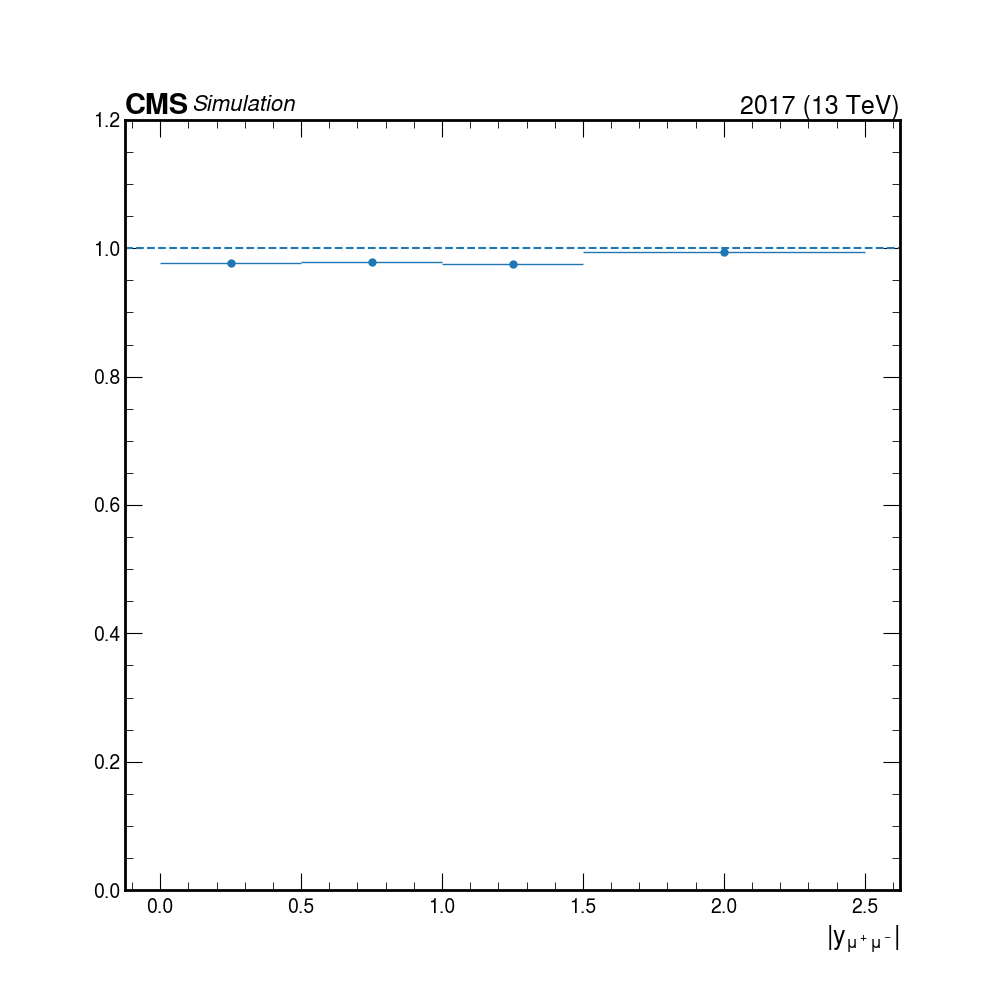
\includegraphics[width=0.44\textwidth]{figures/efficiency/eff_cuts_dimu_rap_2017.png}}}\hfill\\
  \subfloat[][]{\label{subfig:eff_cuts_dimu_2D_2017}%
  \fbox{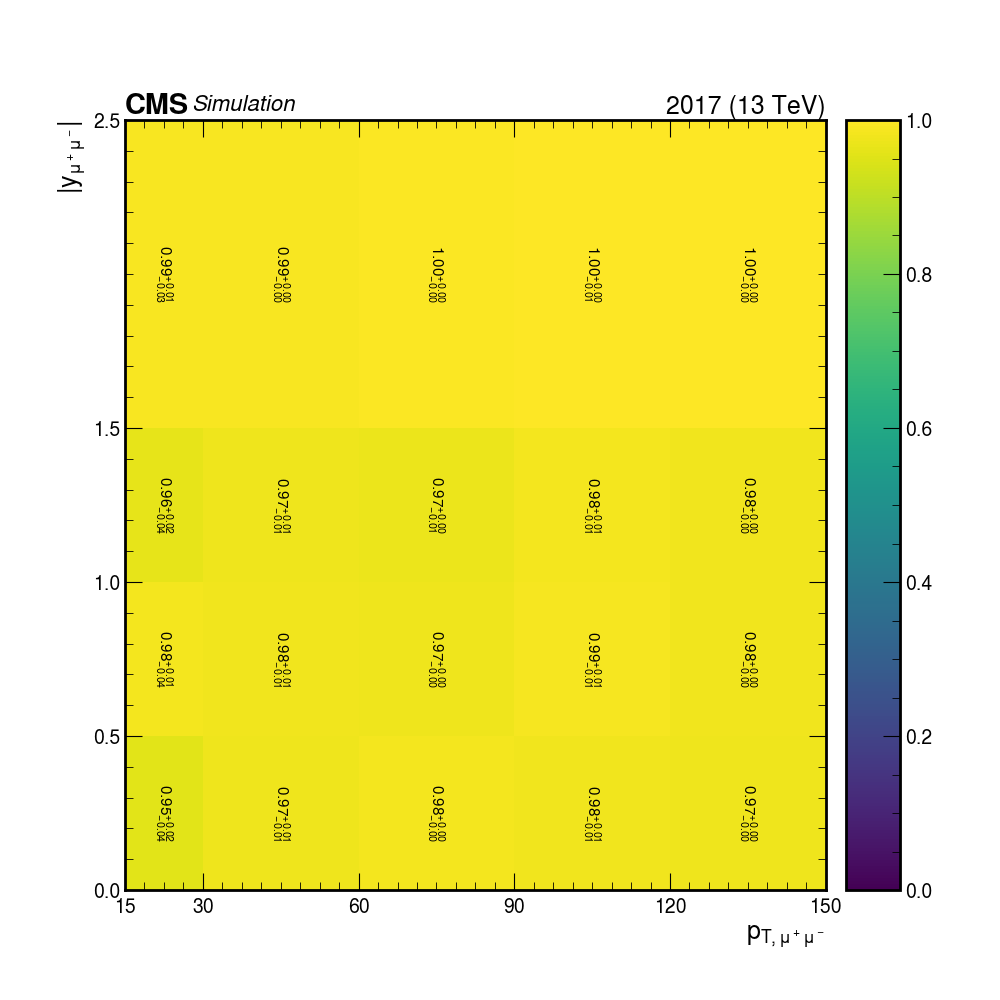
\includegraphics[width=0.44\textwidth]{figures/efficiency/eff_cuts_dimu_2017.png}}}\\
  \legend{$\Upsilon$ selection cuts efficiency extracted from the 2017 MC data sample. This efficiency is given with respect to the dimuon $p_T$ in (a), $y$ in (b), and in both $p_T$ and $y$ in (c). In (a) and (b). The horizontal dashed line is set to the upper limit of the efficiency.}
\end{figure}

\begin{figure}[H]{15cm}
  \caption{D$^*$ selection cuts efficiency of the selected associated $\Upsilon +$ D$^*$ extracted from 2017 MC sample.}
  \label{fig:eff_cuts_dstar_2017}
  \subfloat[][]{\label{subfig:eff_cuts_dstar_pt_2017}%
    \fbox{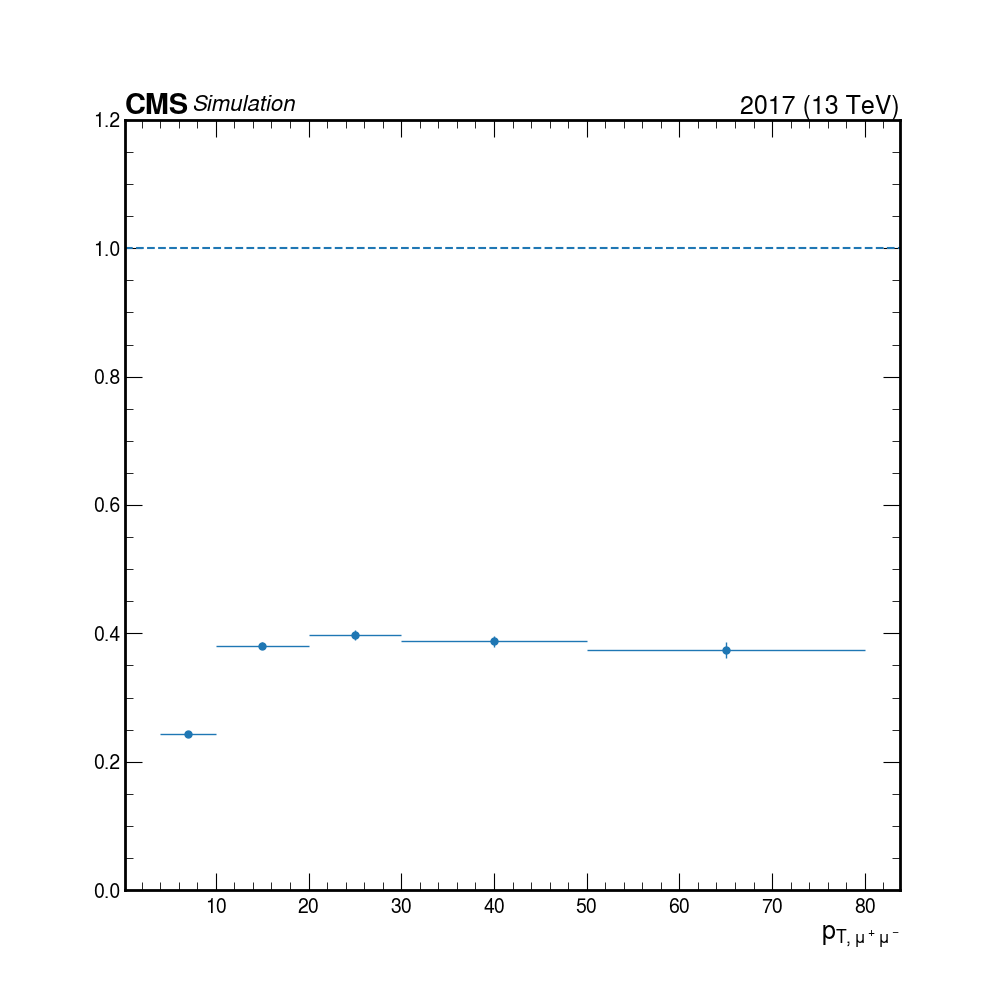
\includegraphics[width=0.44\textwidth]{figures/efficiency/eff_cuts_dstar_pt_2017.png}}}\hfill
  \subfloat[][]{\label{subfig:eff_cuts_dstar_rap_2017}%
    \fbox{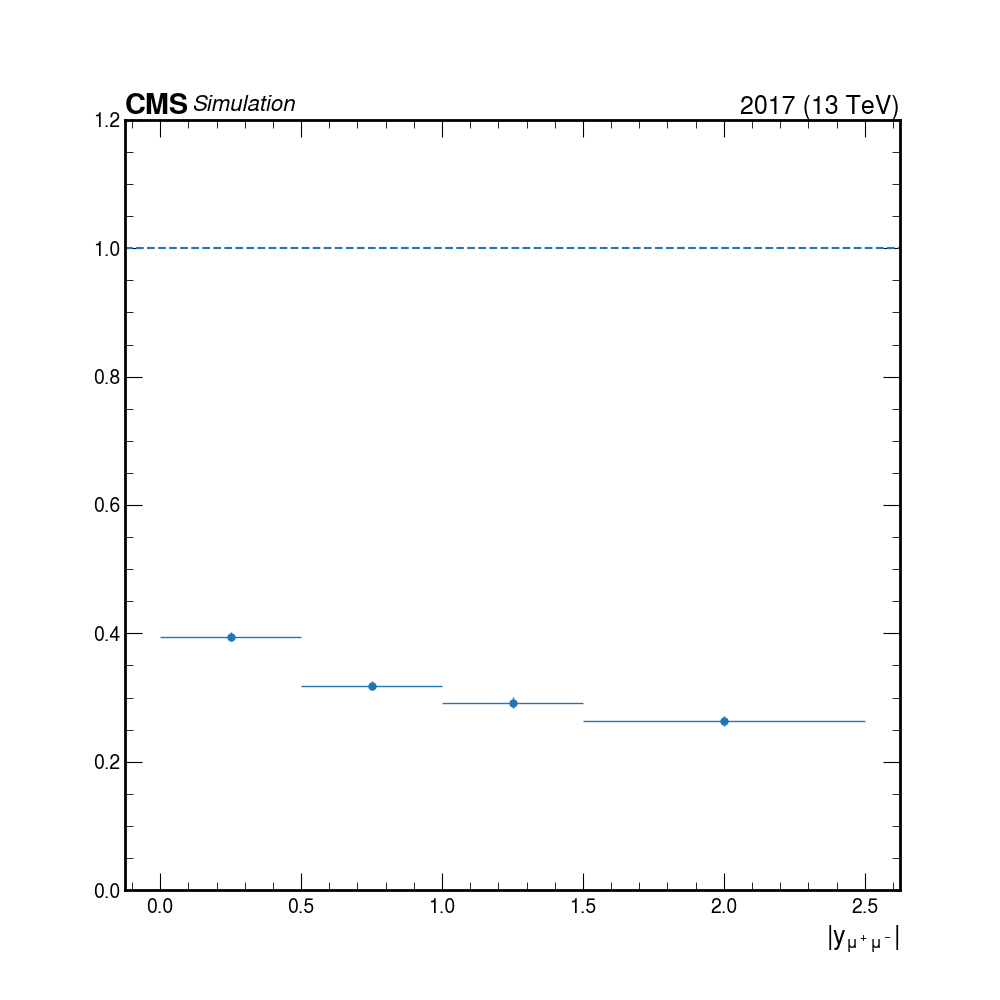
\includegraphics[width=0.44\textwidth]{figures/efficiency/eff_cuts_dstar_rap_2017.png}}}\hfill\\
  \subfloat[][]{\label{subfig:eff_cuts_dstar_2D_2017}%
    \fbox{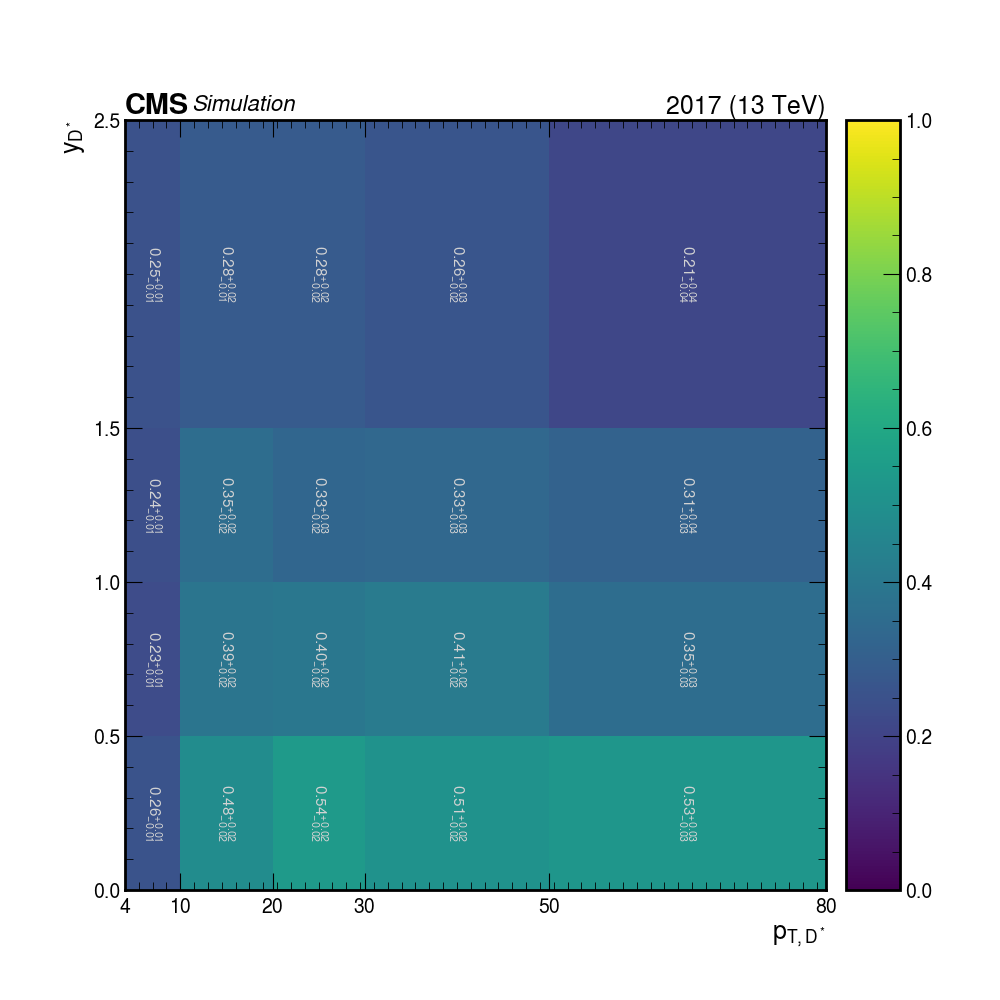
\includegraphics[width=0.44\textwidth]{figures/efficiency/eff_cuts_dstar_2017.png}}}\\
  \legend{D$^*$ selection cuts efficiency extracted from the 2017 MC data sample. This efficiency is given with respect to the D$^*$ $p_T$ in (a), $y$ in (b), and in both $p_T$ and $y$ in (c). In (a) and (b). The horizontal dashed line is set to the upper limit of the efficiency.}
\end{figure}

\begin{figure}[H]{15cm}
  \caption{Trigger efficiency of the selected associated $\Upsilon +$ D$^*$ extracted from 2017 MC sample.}
  \label{fig:eff_trigger_2017}
  \subfloat[][]{\label{subfig:eff_trigger_pt_2017}%
    \fbox{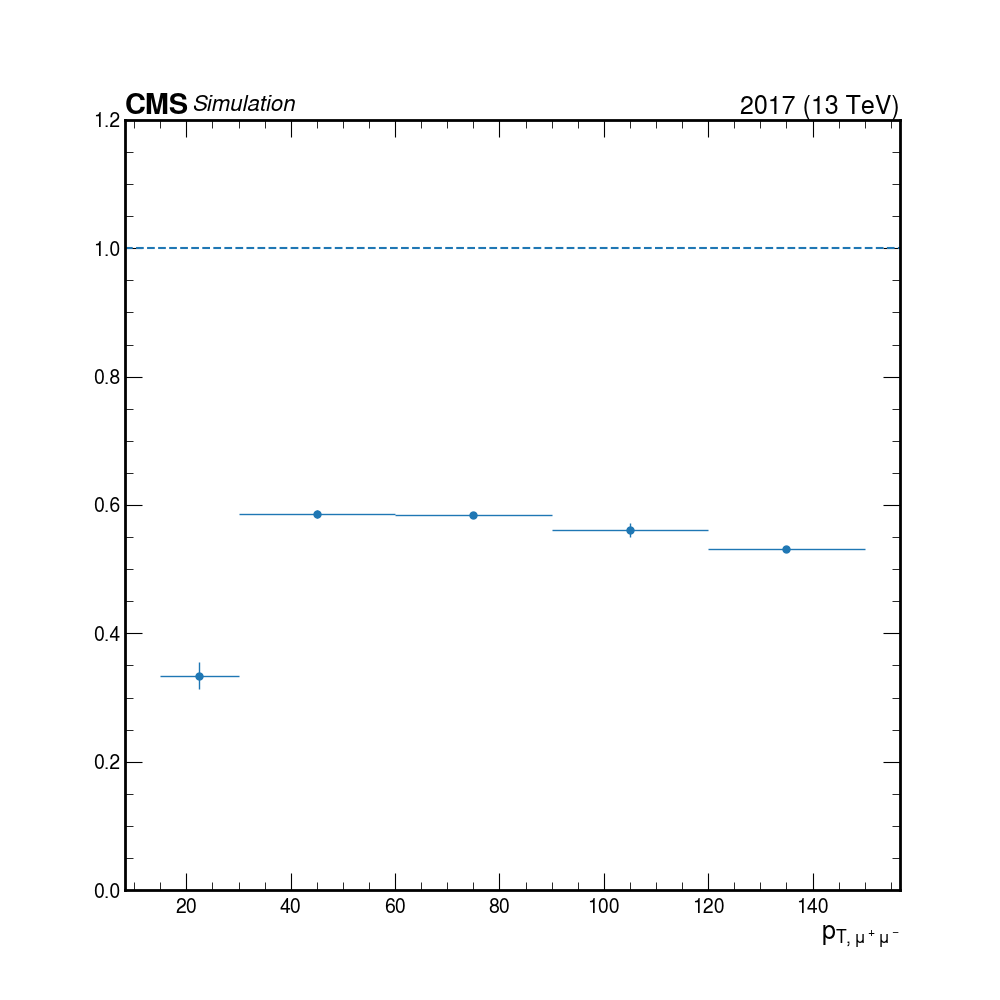
\includegraphics[width=0.44\textwidth]{figures/efficiency/eff_trigger_pt_2017.png}}}\hfill
  \subfloat[][]{\label{subfig:eff_trigger_rap_2017}%
    \fbox{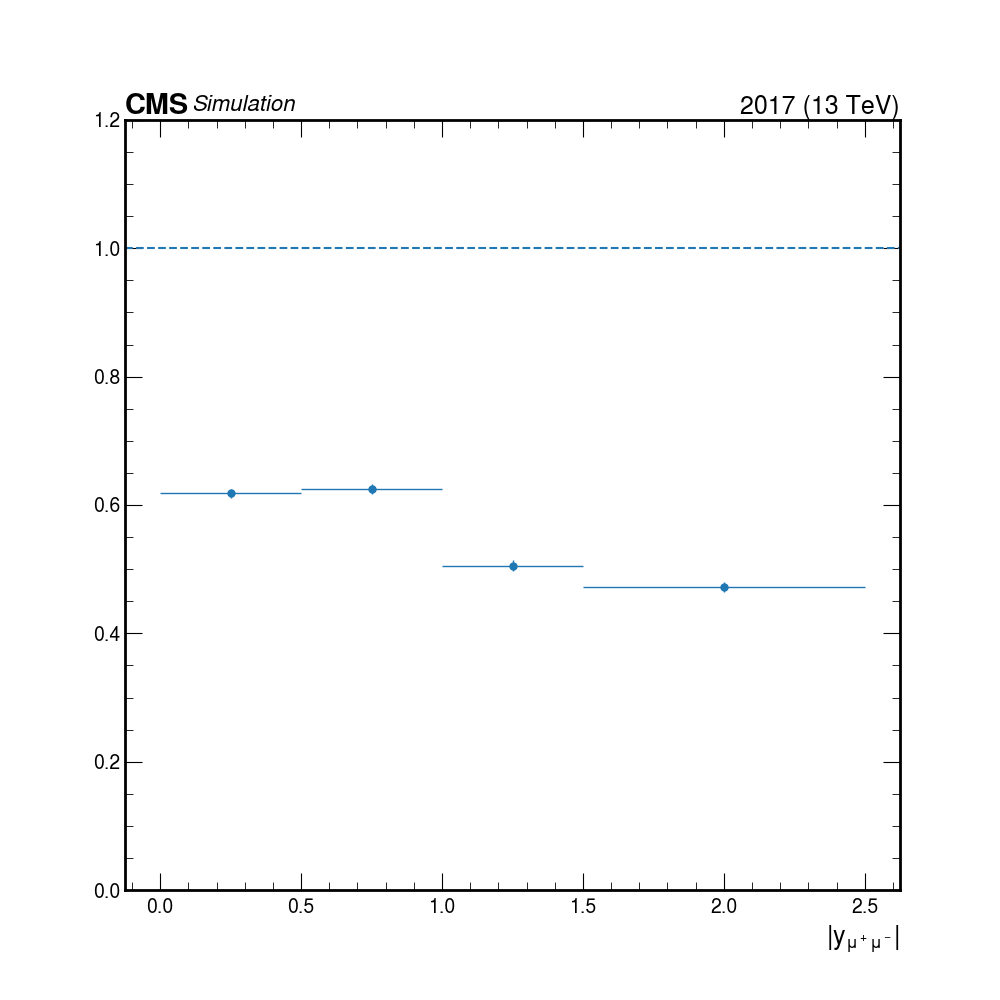
\includegraphics[width=0.44\textwidth]{figures/efficiency/eff_trigger_rap_2017.png}}}\hfill\\
  \subfloat[][]{\label{subfig:eff_trigger_2D_2017}%
    \fbox{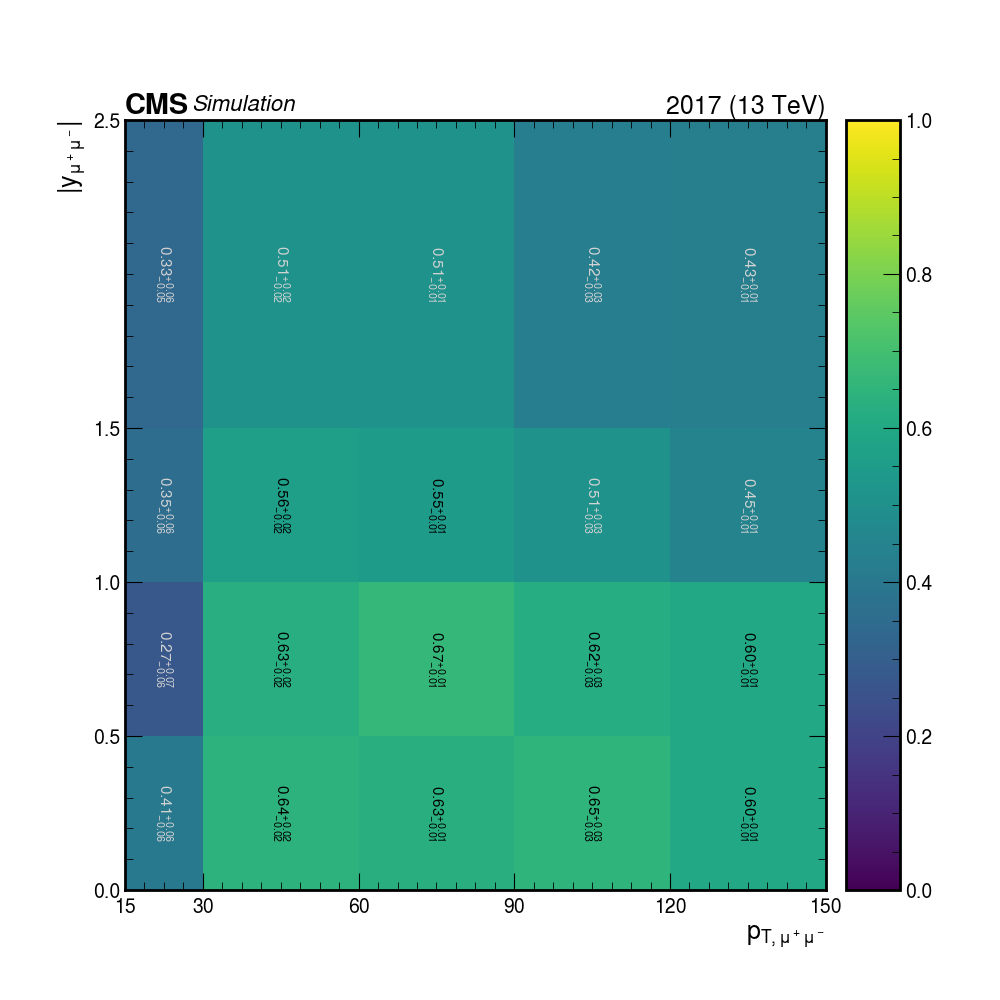
\includegraphics[width=0.44\textwidth]{figures/efficiency/eff_trigger_2017.png}}}\\
  \legend{Trigger efficiency extracted from the 2017 MC data sample. This efficiency is given with respect to the dimuon $p_T$ in (a), $y$ in (b), and in both $p_T$ and $y$ in (c). In (a) and (b). The horizontal dashed line is set to the upper limit of the efficiency.}
\end{figure}

\begin{figure}[H]{15cm}
  \caption{Trigger efficiency of the selected associated $\Upsilon +$ D$^*$ extracted from 2017 MC sample.}
  \label{fig:eff_asso_2017}
  \subfloat[][]{\label{subfig:eff_asso_pt_2017}%
    \fbox{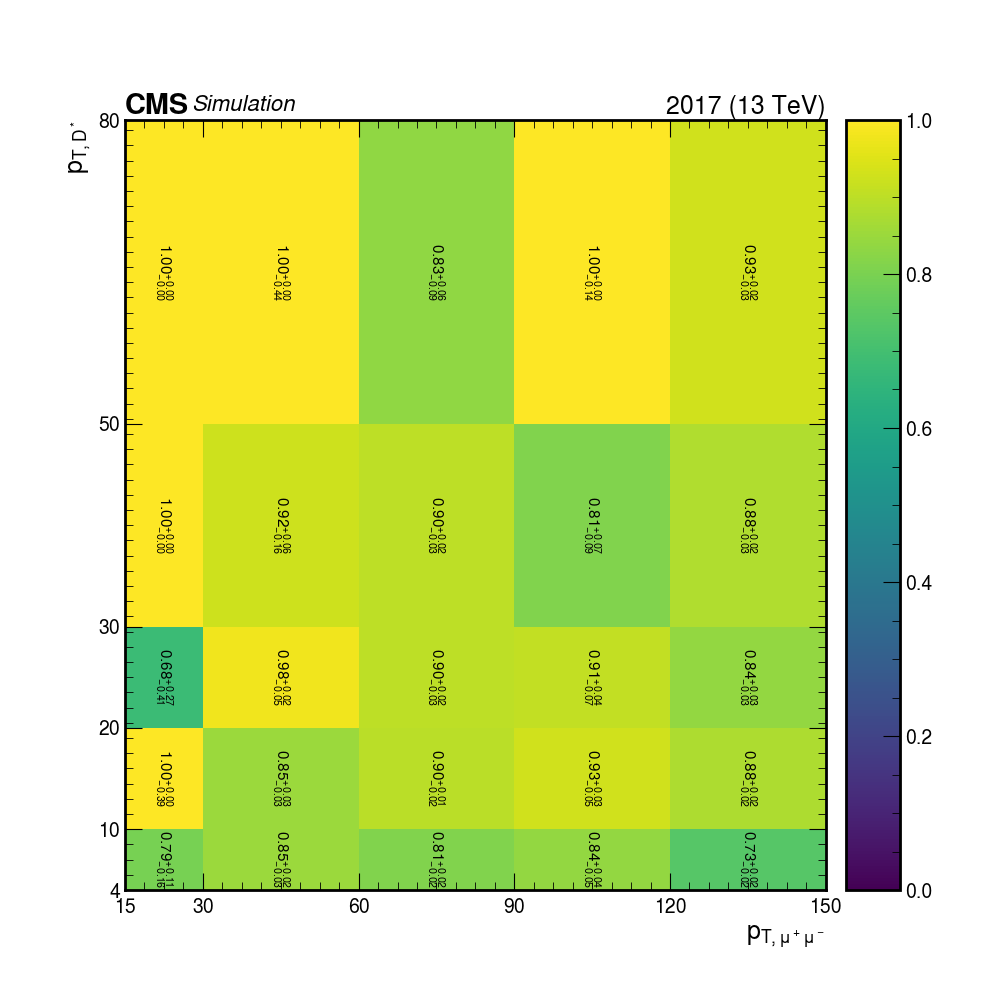
\includegraphics[width=0.44\textwidth]{figures/efficiency/eff_asso_pt_2017.png}}}\hfill
  \subfloat[][]{\label{subfig:eff_asso_rap_2017}%
    \fbox{\includegraphics[width=0.44\textwidth]{figures/efficiency/eff_asso_rap_2017.png}}}\hfill\\
  \legend{Association efficiency extracted from the 2017 MC data sample. The efficiency maps are given with respect to the dimuon and D$^*$ $p_T$ in (a) and $y$ in (b).}
\end{figure}

\clearpage

\section{Efficiencies for sample 2018}

\begin{figure}[H]{15cm}
  \caption{$\Upsilon$ acceptance of the selected associated $\Upsilon +$ D$^*$ extracted from 2018 MC sample.}
  \label{fig:acc_dimu_2018}
  \subfloat[][]{\label{subfig:acc_dimu_pt_2018}%
    \fbox{\includegraphics[width=0.44\textwidth]{figures/efficiency/acc_dimu_pt_2018.png}}}\hfill
  \subfloat[][]{\label{subfig:acc_dimu_rap_2018}%
    \fbox{\includegraphics[width=0.44\textwidth]{figures/efficiency/acc_dimu_rap_2018.png}}}\hfill\\
  \subfloat[][]{\label{subfig:acc_dimu_2D_2018}%
    \fbox{\includegraphics[width=0.44\textwidth]{figures/efficiency/acc_dimu_2018.png}}}\\
  \legend{$\Upsilon$ acceptance extracted from the 2018 MC data sample. The acceptance is given with respect to the dimuon $p_T$ in (a), $y$ in (b), and in both $p_T$ and $y$ in (c). In (a) and (b). The horizontal dashed line is set to the upper limit of the acceptance, one.}
\end{figure}

\begin{figure}[H]{15cm}
  \caption{D$^*$ acceptance of the selected associated $\Upsilon +$ D$^*$ extracted from 2018 MC sample.}
  \label{fig:acc_dstar_2018}
  \subfloat[][]{\label{subfig:acc_dstar_pt_2018}%
    \fbox{\includegraphics[width=0.44\textwidth]{figures/efficiency/acc_dstar_pt_2018.png}}}\hfill
  \subfloat[][]{\label{subfig:acc_dstar_rap_2018}%
    \fbox{\includegraphics[width=0.44\textwidth]{figures/efficiency/acc_dstar_rap_2018.png}}}\hfill\\
  \subfloat[][]{\label{subfig:acc_dstar_2D_2018}%
    \fbox{\includegraphics[width=0.44\textwidth]{figures/efficiency/acc_dstar_2018.png}}}\\
  \legend{D$^*$ acceptance extracted from the 2018 MC data sample. The acceptance is given with respect to the reconstructed D$^*$ $p_T$ in (a), $y$ in (b), and in both $p_T$ and $y$ in (c). In (a) and (b). The horizontal dashed line is set to the upper limit of the acceptance, one.}
\end{figure}

\begin{figure}[H]{15cm}
  \caption{$\Upsilon$ selection cuts efficiency of the selected associated $\Upsilon +$ D$^*$ extracted from 2018 MC sample.}
  \label{fig:eff_cuts_dimu_2018}
  \subfloat[][]{\label{subfig:eff_cuts_dimu_pt_2018}%
  \fbox{\includegraphics[width=0.44\textwidth]{figures/efficiency/eff_cuts_dimu_pt_2018.png}}}\hfill
  \subfloat[][]{\label{subfig:eff_cuts_dimu_rap_2018}%
  \fbox{\includegraphics[width=0.44\textwidth]{figures/efficiency/eff_cuts_dimu_rap_2018.png}}}\hfill\\
  \subfloat[][]{\label{subfig:eff_cuts_dimu_2D_2018}%
  \fbox{\includegraphics[width=0.44\textwidth]{figures/efficiency/eff_cuts_dimu_2018.png}}}\\
  \legend{$\Upsilon$ selection cuts efficiency extracted from the 2018 MC data sample. This efficiency is given with respect to the dimuon $p_T$ in (a), $y$ in (b), and in both $p_T$ and $y$ in (c). In (a) and (b). The horizontal dashed line is set to the upper limit of the efficiency.}
\end{figure}

\begin{figure}[H]{15cm}
  \caption{D$^*$ selection cuts efficiency of the selected associated $\Upsilon +$ D$^*$ extracted from 2018 MC sample.}
  \label{fig:eff_cuts_dstar_2018}
  \subfloat[][]{\label{subfig:eff_cuts_dstar_pt_2018}%
    \fbox{\includegraphics[width=0.44\textwidth]{figures/efficiency/eff_cuts_dstar_pt_2018.png}}}\hfill
  \subfloat[][]{\label{subfig:eff_cuts_dstar_rap_2018}%
    \fbox{\includegraphics[width=0.44\textwidth]{figures/efficiency/eff_cuts_dstar_rap_2018.png}}}\hfill\\
  \subfloat[][]{\label{subfig:eff_cuts_dstar_2D_2018}%
    \fbox{\includegraphics[width=0.44\textwidth]{figures/efficiency/eff_cuts_dstar_2018.png}}}\\
  \legend{D$^*$ selection cuts efficiency extracted from the 2018 MC data sample. This efficiency is given with respect to the D$^*$ $p_T$ in (a), $y$ in (b), and in both $p_T$ and $y$ in (c). In (a) and (b). The horizontal dashed line is set to the upper limit of the efficiency.}
\end{figure}

\begin{figure}[H]{15cm}
  \caption{Trigger efficiency of the selected associated $\Upsilon +$ D$^*$ extracted from 2018 MC sample.}
  \label{fig:eff_trigger_2018}
  \subfloat[][]{\label{subfig:eff_trigger_pt_2018}%
    \fbox{\includegraphics[width=0.44\textwidth]{figures/efficiency/eff_trigger_pt_2018.png}}}\hfill
  \subfloat[][]{\label{subfig:eff_trigger_rap_2018}%
    \fbox{\includegraphics[width=0.44\textwidth]{figures/efficiency/eff_trigger_rap_2018.png}}}\hfill\\
  \subfloat[][]{\label{subfig:eff_trigger_2D_2018}%
    \fbox{\includegraphics[width=0.44\textwidth]{figures/efficiency/eff_trigger_2018.png}}}\\
  \legend{Trigger efficiency extracted from the 2018 MC data sample. This efficiency is given with respect to the dimuon $p_T$ in (a), $y$ in (b), and in both $p_T$ and $y$ in (c). In (a) and (b). The horizontal dashed line is set to the upper limit of the efficiency.}
\end{figure}

\begin{figure}[H]{15cm}
  \caption{Trigger efficiency of the selected associated $\Upsilon +$ D$^*$ extracted from 2018 MC sample.}
  \label{fig:eff_asso_2018}
  \subfloat[][]{\label{subfig:eff_asso_pt_2018}%
    \fbox{\includegraphics[width=0.44\textwidth]{figures/efficiency/eff_asso_pt_2018.png}}}\hfill
  \subfloat[][]{\label{subfig:eff_asso_rap_2018}%
    \fbox{\includegraphics[width=0.44\textwidth]{figures/efficiency/eff_asso_rap_2018.png}}}\hfill\\
  \legend{Association efficiency extracted from the 2018 MC data sample. The efficiency maps are given with respect to the dimuon and D$^*$ $p_T$ in (a) and $y$ in (b).}
\end{figure}

\postextualchapter{Kinematic Distributions}\label{app:dists}

\section{Distributions for sample 2016APV}

\begin{figure}[!htm]{15cm}
  \caption{Dimuon distributions for 2016APV sample}
  \label{fig:dimu_dists_2016APV}
  \subfloat[][]{\label{subfig:dimu_pt_2016APV}%
    \fbox{\includegraphics[width=0.47\textwidth]{figures/comparison/2016APV/dimu_pt_log_2016APV.png}}}\hfill
  \subfloat[][]{\label{subfig:dimu_rap_2016APV}%
    \fbox{\includegraphics[width=0.47\textwidth]{figures/comparison/2016APV/dimu_rap_2016APV.png}}}\\
  \subfloat[][]{\label{subfig:dimu_phi_2016APV}%
    \fbox{\includegraphics[width=0.47\textwidth]{figures/comparison/2016APV/dimu_phi_2016APV.png}}}\hfill
  \subfloat[][]{\label{subfig:dimu_mass_2016APV}%
    \fbox{\includegraphics[width=0.47\textwidth]{figures/comparison/2016APV/dimu_mass_2016APV.png}}}\\
  \legend{p$_T$ (a), $y$ (b) and $\phi$ (c), invariant mass (d) distributions for the $\Upsilon$ candidate using the 2016APV data sample. The black dots represent the CMS Run 2 data, while the blue distribution represent the signal DPS MC simulation and the orange one the signal SPS MC simulation.}
\end{figure}

\begin{figure}[!htm]{15cm}
  \caption{D$^*$ distributions for 2016APV sample}
  \label{fig:dstar_dists_2016APV}
  \subfloat[][]{\label{subfig:dstar_pt_2016APV}%
    \fbox{\includegraphics[width=0.47\textwidth]{figures/comparison/2016APV/dstar_pt_log_2016APV.png}}}\hfill
  \subfloat[][]{\label{subfig:dstar_rap_2016APV}%
    \fbox{\includegraphics[width=0.47\textwidth]{figures/comparison/2016APV/dstar_rap_2016APV.png}}}\\
  \subfloat[][]{\label{subfig:dstar_phi_2016APV}%
    \fbox{\includegraphics[width=0.47\textwidth]{figures/comparison/2016APV/dstar_phi_2016APV.png}}}\hfill
  \subfloat[][]{\label{subfig:dstar_deltam_2016APV}%
    \fbox{\includegraphics[width=0.47\textwidth]{figures/comparison/2016APV/dstar_deltamr_2016APV.png}}}\\
  \legend{p$_T$ (a), $y$ (b), $\phi$ (c) and $\Delta m$ (d) distributions for the D$^*$ candidate using the 2016APV data sample. The black dots represent the CMS Run 2 data, while the blue distribution represent the signal DPS MC simulation and the orange one the signal SPS MC simulation.}
\end{figure}

\begin{figure}[!htm]{15cm}
  \caption{D$^0$ distributions for 2016APV sample}
  \label{fig:dstar_d0_dists_2016APV}
  \subfloat[][]{\label{subfig:dstar_d0_pt_2016APV}%
    \fbox{\includegraphics[width=0.42\textwidth]{figures/comparison/2016APV/dstar_d0_pt_log_2016APV.png}}}\hfill
  \subfloat[][]{\label{subfig:dstar_d0_eta_2016APV}%
    \fbox{\includegraphics[width=0.42\textwidth]{figures/comparison/2016APV/dstar_d0_eta_2016APV.png}}}\\
    \subfloat[][]{\label{subfig:dstar_d0_phi_2016APV}%
    \fbox{\includegraphics[width=0.42\textwidth]{figures/comparison/2016APV/dstar_d0_phi_2016APV.png}}}\hfill
  \subfloat[][]{\label{subfig:dstar_d0_mass_2016APV}%
    \fbox{\includegraphics[width=0.42\textwidth]{figures/comparison/2016APV/dstar_d0_dlSig_2016APV.png}}}\\
  \subfloat[][]{\label{subfig:dstar_d0_cosphi_2016APV}%
    \fbox{\includegraphics[width=0.42\textwidth]{figures/comparison/2016APV/dstar_d0_cosphi_2016APV.png}}}\hfill
  \subfloat[][]{\label{subfig:dstar_d0_dlSig_2016APV}%
    \fbox{\includegraphics[width=0.42\textwidth]{figures/comparison/2016APV/dstar_d0_dlSig_2016APV.png}}}\\
  \legend{p$_T$ (a), $\eta$ (b), $\phi$ (c), invariant mass (d), $\cos{\alpha}$ (e) and dl$_{sig}$ (f) distributions for the D$^0$ using the 2016APV data sample. The black dots represent the CMS Run 2 data, while the blue distribution represent the signal DPS MC simulation and the orange one the signal SPS MC simulation.}
\end{figure}

\begin{figure}[!htm]{15cm}
  \caption{Associated $\Upsilon$ and D$^*$ distributions for 2016APV sample}
  \label{fig:dimudstar_dists_2016APV}
  \subfloat[][]{\label{subfig:dimudstar_pt_2016APV}%
    \fbox{\includegraphics[width=0.47\textwidth]{figures/comparison/2016APV/pt_log_2016APV.png}}}\hfill
  \subfloat[][]{\label{subfig:dimudstar_rap_2016APV}%
    \fbox{\includegraphics[width=0.47\textwidth]{figures/comparison/2016APV/rap_2016APV.png}}}\\
  \subfloat[][]{\label{subfig:dimudstar_phi_2016APV}%
    \fbox{\includegraphics[width=0.47\textwidth]{figures/comparison/2016APV/phi_2016APV.png}}}\hfill
  \subfloat[][]{\label{subfig:dimudstar_mass_2016APV}%
    \fbox{\includegraphics[width=0.47\textwidth]{figures/comparison/2016APV/mass_2016APV.png}}}\\
  \legend{p$_T$ (a), $y$ (b), $\phi$ (c) and invariant mass (d) distributions for the associated $\Upsilon$ and D$^*$ candidate using the 2016APV data sample. The black dots represent the CMS Run 2 data, while the blue distribution represent the signal DPS MC simulation and the orange one the signal SPS MC simulation.}
\end{figure}

\begin{figure}[!htm]{15cm}
  \caption{Associated $\Upsilon$ and D$^*$ $\Delta p_T$, $\Delta$y and $\Delta\phi$ distributions for 2016APV sample}
  \label{fig:dimudstar_delta_dists_2016APV}
  \subfloat[][]{\label{subfig:dimudstar_deltapt_2016APV}%
    \fbox{\includegraphics[width=0.47\textwidth]{figures/comparison/2016APV/deltapt_log_2016APV.png}}}\hfill
  \subfloat[][]{\label{subfig:dimudstar_deltarap_2016APV}%
    \fbox{\includegraphics[width=0.47\textwidth]{figures/comparison/2016APV/deltarap_2016APV.png}}}\\
  \subfloat[][]{\label{subfig:dimudstar_deltaphi_2016APV}%
    \fbox{\includegraphics[width=0.47\textwidth]{figures/comparison/2016APV/deltaphi_2016APV.png}}}\\
  \legend{$\Delta p_T$ (a), $\Delta y$ (b) and $\Delta \phi$ (c) distributions for the assocuated $\Upsilon$ and D$^*$ candidate using the 2016APV data sample. The black dots represent the CMS Run 2 data, while the blue distribution represent the signal DPS MC simulation and the orange one the signal SPS MC simulation.}
\end{figure}

\clearpage

\section{Distributions for sample 2016}

\begin{figure}[!htm]{15cm}
  \caption{Dimuon distributions for 2016 sample}
  \label{fig:dimu_dists_2016}
  \subfloat[][]{\label{subfig:dimu_pt_2016}%
    \fbox{\includegraphics[width=0.47\textwidth]{figures/comparison/2016/dimu_pt_log_2016.png}}}\hfill
  \subfloat[][]{\label{subfig:dimu_rap_2016}%
    \fbox{\includegraphics[width=0.47\textwidth]{figures/comparison/2016/dimu_rap_2016.png}}}\\
  \subfloat[][]{\label{subfig:dimu_phi_2016}%
    \fbox{\includegraphics[width=0.47\textwidth]{figures/comparison/2016/dimu_phi_2016.png}}}\hfill
  \subfloat[][]{\label{subfig:dimu_mass_2016}%
    \fbox{\includegraphics[width=0.47\textwidth]{figures/comparison/2016/dimu_mass_2016.png}}}\\
  \legend{p$_T$ (a), $y$ (b) and $\phi$ (c), invariant mass (d) distributions for the $\Upsilon$ candidate using the 2016 data sample. The black dots represent the CMS Run 2 data, while the blue distribution represent the signal DPS MC simulation and the orange one the signal SPS MC simulation.}
\end{figure}

\begin{figure}[!htm]{15cm}
  \caption{D$^*$ distributions for 2016 sample}
  \label{fig:dstar_dists_2016}
  \subfloat[][]{\label{subfig:dstar_pt_2016}%
    \fbox{\includegraphics[width=0.47\textwidth]{figures/comparison/2016/dstar_pt_log_2016.png}}}\hfill
  \subfloat[][]{\label{subfig:dstar_rap_2016}%
    \fbox{\includegraphics[width=0.47\textwidth]{figures/comparison/2016/dstar_rap_2016.png}}}\\
  \subfloat[][]{\label{subfig:dstar_phi_2016}%
    \fbox{\includegraphics[width=0.47\textwidth]{figures/comparison/2016/dstar_phi_2016.png}}}\hfill
  \subfloat[][]{\label{subfig:dstar_deltam_2016}%
    \fbox{\includegraphics[width=0.47\textwidth]{figures/comparison/2016/dstar_deltamr_2016.png}}}\\
  \legend{p$_T$ (a), $y$ (b), $\phi$ (c) and $\Delta m$ (d) distributions for the D$^*$ candidate using the 2016 data sample. The black dots represent the CMS Run 2 data, while the blue distribution represent the signal DPS MC simulation and the orange one the signal SPS MC simulation.}
\end{figure}

\begin{figure}[!htm]{15cm}
  \caption{D$^0$ distributions for 2016 sample}
  \label{fig:dstar_d0_dists_2016}
  \subfloat[][]{\label{subfig:dstar_d0_pt_2016}%
    \fbox{\includegraphics[width=0.42\textwidth]{figures/comparison/2016/dstar_d0_pt_log_2016.png}}}\hfill
  \subfloat[][]{\label{subfig:dstar_d0_eta_2016}%
    \fbox{\includegraphics[width=0.42\textwidth]{figures/comparison/2016/dstar_d0_eta_2016.png}}}\\
    \subfloat[][]{\label{subfig:dstar_d0_phi_2016}%
    \fbox{\includegraphics[width=0.42\textwidth]{figures/comparison/2016/dstar_d0_phi_2016.png}}}\hfill
  \subfloat[][]{\label{subfig:dstar_d0_mass_2016}%
    \fbox{\includegraphics[width=0.42\textwidth]{figures/comparison/2016/dstar_d0_dlSig_2016.png}}}\\
  \subfloat[][]{\label{subfig:dstar_d0_cosphi_2016}%
    \fbox{\includegraphics[width=0.42\textwidth]{figures/comparison/2016/dstar_d0_cosphi_2016.png}}}\hfill
  \subfloat[][]{\label{subfig:dstar_d0_dlSig_2016}%
    \fbox{\includegraphics[width=0.42\textwidth]{figures/comparison/2016/dstar_d0_dlSig_2016.png}}}\\
  \legend{p$_T$ (a), $\eta$ (b), $\phi$ (c), invariant mass (d), $\cos{\alpha}$ (e) and dl$_{sig}$ (f) distributions for the D$^0$ using the 2016 data sample. The black dots represent the CMS Run 2 data, while the blue distribution represent the signal DPS MC simulation and the orange one the signal SPS MC simulation.}
\end{figure}

\begin{figure}[!htm]{15cm}
  \caption{Associated $\Upsilon$ and D$^*$ distributions for 2016 sample}
  \label{fig:dimudstar_dists_2016}
  \subfloat[][]{\label{subfig:dimudstar_pt_2016}%
    \fbox{\includegraphics[width=0.47\textwidth]{figures/comparison/2016/pt_log_2016.png}}}\hfill
  \subfloat[][]{\label{subfig:dimudstar_rap_2016}%
    \fbox{\includegraphics[width=0.47\textwidth]{figures/comparison/2016/rap_2016.png}}}\\
  \subfloat[][]{\label{subfig:dimudstar_phi_2016}%
    \fbox{\includegraphics[width=0.47\textwidth]{figures/comparison/2016/phi_2016.png}}}\hfill
  \subfloat[][]{\label{subfig:dimudstar_mass_2016}%
    \fbox{\includegraphics[width=0.47\textwidth]{figures/comparison/2016/mass_2016.png}}}\\
  \legend{p$_T$ (a), $y$ (b), $\phi$ (c) and invariant mass (d) distributions for the associated $\Upsilon$ and D$^*$ candidate using the 2016 data sample. The black dots represent the CMS Run 2 data, while the blue distribution represent the signal DPS MC simulation and the orange one the signal SPS MC simulation.}
\end{figure}

\begin{figure}[!htm]{15cm}
  \caption{Associated $\Upsilon$ and D$^*$ $\Delta p_T$, $\Delta$y and $\Delta\phi$ distributions for 2016 sample}
  \label{fig:dimudstar_delta_dists_2016}
  \subfloat[][]{\label{subfig:dimudstar_deltapt_2016}%
    \fbox{\includegraphics[width=0.47\textwidth]{figures/comparison/2016/deltapt_log_2016.png}}}\hfill
  \subfloat[][]{\label{subfig:dimudstar_deltarap_2016}%
    \fbox{\includegraphics[width=0.47\textwidth]{figures/comparison/2016/deltarap_2016.png}}}\\
  \subfloat[][]{\label{subfig:dimudstar_deltaphi_2016}%
    \fbox{\includegraphics[width=0.47\textwidth]{figures/comparison/2016/deltaphi_2016.png}}}\\
  \legend{$\Delta p_T$ (a), $\Delta y$ (b) and $\Delta \phi$ (c) distributions for the assocuated $\Upsilon$ and D$^*$ candidate using the 2016 data sample. The black dots represent the CMS Run 2 data, while the blue distribution represent the signal DPS MC simulation and the orange one the signal SPS MC simulation.}
\end{figure}

\clearpage

\section{Distributions for sample 2017}

\begin{figure}[!htm]{15cm}
  \caption{Dimuon distributions for 2017 sample}
  \label{fig:dimu_dists_2017}
  \subfloat[][]{\label{subfig:dimu_pt_2017}%
    \fbox{\includegraphics[width=0.47\textwidth]{figures/comparison/2017/dimu_pt_log_2017.png}}}\hfill
  \subfloat[][]{\label{subfig:dimu_rap_2017}%
    \fbox{\includegraphics[width=0.47\textwidth]{figures/comparison/2017/dimu_rap_2017.png}}}\\
  \subfloat[][]{\label{subfig:dimu_phi_2017}%
    \fbox{\includegraphics[width=0.47\textwidth]{figures/comparison/2017/dimu_phi_2017.png}}}\hfill
  \subfloat[][]{\label{subfig:dimu_mass_2017}%
    \fbox{\includegraphics[width=0.47\textwidth]{figures/comparison/2017/dimu_mass_2017.png}}}\\
  \legend{p$_T$ (a), $y$ (b) and $\phi$ (c), invariant mass (d) distributions for the $\Upsilon$ candidate using the 2017 data sample. The black dots represent the CMS Run 2 data, while the blue distribution represent the signal DPS MC simulation and the orange one the signal SPS MC simulation.}
\end{figure}

\begin{figure}[!htm]{15cm}
  \caption{D$^*$ distributions for 2017 sample}
  \label{fig:dstar_dists_2017}
  \subfloat[][]{\label{subfig:dstar_pt_2017}%
    \fbox{\includegraphics[width=0.47\textwidth]{figures/comparison/2017/dstar_pt_log_2017.png}}}\hfill
  \subfloat[][]{\label{subfig:dstar_rap_2017}%
    \fbox{\includegraphics[width=0.47\textwidth]{figures/comparison/2017/dstar_rap_2017.png}}}\\
  \subfloat[][]{\label{subfig:dstar_phi_2017}%
    \fbox{\includegraphics[width=0.47\textwidth]{figures/comparison/2017/dstar_phi_2017.png}}}\hfill
  \subfloat[][]{\label{subfig:dstar_deltam_2017}%
    \fbox{\includegraphics[width=0.47\textwidth]{figures/comparison/2017/dstar_deltamr_2017.png}}}\\
  \legend{p$_T$ (a), $y$ (b), $\phi$ (c) and $\Delta m$ (d) distributions for the D$^*$ candidate using the 2017 data sample. The black dots represent the CMS Run 2 data, while the blue distribution represent the signal DPS MC simulation and the orange one the signal SPS MC simulation.}
\end{figure}

\begin{figure}[!htm]{15cm}
  \caption{D$^0$ distributions for 2017 sample}
  \label{fig:dstar_d0_dists_2017}
  \subfloat[][]{\label{subfig:dstar_d0_pt_2017}%
    \fbox{\includegraphics[width=0.42\textwidth]{figures/comparison/2017/dstar_d0_pt_log_2017.png}}}\hfill
  \subfloat[][]{\label{subfig:dstar_d0_eta_2017}%
    \fbox{\includegraphics[width=0.42\textwidth]{figures/comparison/2017/dstar_d0_eta_2017.png}}}\\
    \subfloat[][]{\label{subfig:dstar_d0_phi_2017}%
    \fbox{\includegraphics[width=0.42\textwidth]{figures/comparison/2017/dstar_d0_phi_2017.png}}}\hfill
  \subfloat[][]{\label{subfig:dstar_d0_mass_2017}%
    \fbox{\includegraphics[width=0.42\textwidth]{figures/comparison/2017/dstar_d0_dlSig_2017.png}}}\\
  \subfloat[][]{\label{subfig:dstar_d0_cosphi_2017}%
    \fbox{\includegraphics[width=0.42\textwidth]{figures/comparison/2017/dstar_d0_cosphi_2017.png}}}\hfill
  \subfloat[][]{\label{subfig:dstar_d0_dlSig_2017}%
    \fbox{\includegraphics[width=0.42\textwidth]{figures/comparison/2017/dstar_d0_dlSig_2017.png}}}\\
  \legend{p$_T$ (a), $\eta$ (b), $\phi$ (c), invariant mass (d), $\cos{\alpha}$ (e) and dl$_{sig}$ (f) distributions for the D$^0$ using the 2017 data sample. The black dots represent the CMS Run 2 data, while the blue distribution represent the signal DPS MC simulation and the orange one the signal SPS MC simulation.}
\end{figure}

\begin{figure}[!htm]{15cm}
  \caption{Associated $\Upsilon$ and D$^*$ distributions for 2017 sample}
  \label{fig:dimudstar_dists_2017}
  \subfloat[][]{\label{subfig:dimudstar_pt_2017}%
    \fbox{\includegraphics[width=0.47\textwidth]{figures/comparison/2017/pt_log_2017.png}}}\hfill
  \subfloat[][]{\label{subfig:dimudstar_rap_2017}%
    \fbox{\includegraphics[width=0.47\textwidth]{figures/comparison/2017/rap_2017.png}}}\\
  \subfloat[][]{\label{subfig:dimudstar_phi_2017}%
    \fbox{\includegraphics[width=0.47\textwidth]{figures/comparison/2017/phi_2017.png}}}\hfill
  \subfloat[][]{\label{subfig:dimudstar_mass_2017}%
    \fbox{\includegraphics[width=0.47\textwidth]{figures/comparison/2017/mass_2017.png}}}\\
  \legend{p$_T$ (a), $y$ (b), $\phi$ (c) and invariant mass (d) distributions for the associated $\Upsilon$ and D$^*$ candidate using the 2017 data sample. The black dots represent the CMS Run 2 data, while the blue distribution represent the signal DPS MC simulation and the orange one the signal SPS MC simulation.}
\end{figure}

\begin{figure}[!htm]{15cm}
  \caption{Associated $\Upsilon$ and D$^*$ $\Delta p_T$, $\Delta$y and $\Delta\phi$ distributions for 2017 sample}
  \label{fig:dimudstar_delta_dists_2017}
  \subfloat[][]{\label{subfig:dimudstar_deltapt_2017}%
    \fbox{\includegraphics[width=0.47\textwidth]{figures/comparison/2017/deltapt_log_2017.png}}}\hfill
  \subfloat[][]{\label{subfig:dimudstar_deltarap_2017}%
    \fbox{\includegraphics[width=0.47\textwidth]{figures/comparison/2017/deltarap_2017.png}}}\\
  \subfloat[][]{\label{subfig:dimudstar_deltaphi_2017}%
    \fbox{\includegraphics[width=0.47\textwidth]{figures/comparison/2017/deltaphi_2017.png}}}\\
  \legend{$\Delta p_T$ (a), $\Delta y$ (b) and $\Delta \phi$ (c) distributions for the assocuated $\Upsilon$ and D$^*$ candidate using the 2017 data sample. The black dots represent the CMS Run 2 data, while the blue distribution represent the signal DPS MC simulation and the orange one the signal SPS MC simulation.}
\end{figure}

\clearpage

\section{Distributions for sample 2018}

\begin{figure}[!htm]{15cm}
  \caption{Dimuon distributions for 2018 sample}
  \label{fig:dimu_dists_2018}
  \subfloat[][]{\label{subfig:dimu_pt_2018}%
    \fbox{\includegraphics[width=0.47\textwidth]{figures/comparison/2018/dimu_pt_log_2018.png}}}\hfill
  \subfloat[][]{\label{subfig:dimu_rap_2018}%
    \fbox{\includegraphics[width=0.47\textwidth]{figures/comparison/2018/dimu_rap_2018.png}}}\\
  \subfloat[][]{\label{subfig:dimu_phi_2018}%
    \fbox{\includegraphics[width=0.47\textwidth]{figures/comparison/2018/dimu_phi_2018.png}}}\hfill
  \subfloat[][]{\label{subfig:dimu_mass_2018}%
    \fbox{\includegraphics[width=0.47\textwidth]{figures/comparison/2018/dimu_mass_2018.png}}}\\
  \legend{p$_T$ (a), $y$ (b) and $\phi$ (c), invariant mass (d) distributions for the $\Upsilon$ candidate using the 2018 data sample. The black dots represent the CMS Run 2 data, while the blue distribution represent the signal DPS MC simulation and the orange one the signal SPS MC simulation.}
\end{figure}

\begin{figure}[!htm]{15cm}
  \caption{D$^*$ distributions for 2018 sample}
  \label{fig:dstar_dists_2018}
  \subfloat[][]{\label{subfig:dstar_pt_2018}%
    \fbox{\includegraphics[width=0.47\textwidth]{figures/comparison/2018/dstar_pt_log_2018.png}}}\hfill
  \subfloat[][]{\label{subfig:dstar_rap_2018}%
    \fbox{\includegraphics[width=0.47\textwidth]{figures/comparison/2018/dstar_rap_2018.png}}}\\
  \subfloat[][]{\label{subfig:dstar_phi_2018}%
    \fbox{\includegraphics[width=0.47\textwidth]{figures/comparison/2018/dstar_phi_2018.png}}}\hfill
  \subfloat[][]{\label{subfig:dstar_deltam_2018}%
    \fbox{\includegraphics[width=0.47\textwidth]{figures/comparison/2018/dstar_deltamr_2018.png}}}\\
  \legend{p$_T$ (a), $y$ (b), $\phi$ (c) and $\Delta m$ (d) distributions for the D$^*$ candidate using the 2018 data sample. The black dots represent the CMS Run 2 data, while the blue distribution represent the signal DPS MC simulation and the orange one the signal SPS MC simulation.}
\end{figure}

\begin{figure}[!htm]{15cm}
  \caption{D$^0$ distributions for 2018 sample}
  \label{fig:dstar_d0_dists_2018}
  \subfloat[][]{\label{subfig:dstar_d0_pt_2018}%
    \fbox{\includegraphics[width=0.42\textwidth]{figures/comparison/2018/dstar_d0_pt_log_2018.png}}}\hfill
  \subfloat[][]{\label{subfig:dstar_d0_eta_2018}%
    \fbox{\includegraphics[width=0.42\textwidth]{figures/comparison/2018/dstar_d0_eta_2018.png}}}\\
    \subfloat[][]{\label{subfig:dstar_d0_phi_2018}%
    \fbox{\includegraphics[width=0.42\textwidth]{figures/comparison/2018/dstar_d0_phi_2018.png}}}\hfill
  \subfloat[][]{\label{subfig:dstar_d0_mass_2018}%
    \fbox{\includegraphics[width=0.42\textwidth]{figures/comparison/2018/dstar_d0_dlSig_2018.png}}}\\
  \subfloat[][]{\label{subfig:dstar_d0_cosphi_2018}%
    \fbox{\includegraphics[width=0.42\textwidth]{figures/comparison/2018/dstar_d0_cosphi_2018.png}}}\hfill
  \subfloat[][]{\label{subfig:dstar_d0_dlSig_2018}%
    \fbox{\includegraphics[width=0.42\textwidth]{figures/comparison/2018/dstar_d0_dlSig_2018.png}}}\\
  \legend{p$_T$ (a), $\eta$ (b), $\phi$ (c), invariant mass (d), $\cos{\alpha}$ (e) and dl$_{sig}$ (f) distributions for the D$^0$ using the 2018 data sample. The black dots represent the CMS Run 2 data, while the blue distribution represent the signal DPS MC simulation and the orange one the signal SPS MC simulation.}
\end{figure}

\begin{figure}[!htm]{15cm}
  \caption{Associated $\Upsilon$ and D$^*$ distributions for 2018 sample}
  \label{fig:dimudstar_dists_2018}
  \subfloat[][]{\label{subfig:dimudstar_pt_2018}%
    \fbox{\includegraphics[width=0.47\textwidth]{figures/comparison/2018/pt_log_2018.png}}}\hfill
  \subfloat[][]{\label{subfig:dimudstar_rap_2018}%
    \fbox{\includegraphics[width=0.47\textwidth]{figures/comparison/2018/rap_2018.png}}}\\
  \subfloat[][]{\label{subfig:dimudstar_phi_2018}%
    \fbox{\includegraphics[width=0.47\textwidth]{figures/comparison/2018/phi_2018.png}}}\hfill
  \subfloat[][]{\label{subfig:dimudstar_mass_2018}%
    \fbox{\includegraphics[width=0.47\textwidth]{figures/comparison/2018/mass_2018.png}}}\\
  \legend{p$_T$ (a), $y$ (b), $\phi$ (c) and invariant mass (d) distributions for the associated $\Upsilon$ and D$^*$ candidate using the 2018 data sample. The black dots represent the CMS Run 2 data, while the blue distribution represent the signal DPS MC simulation and the orange one the signal SPS MC simulation.}
\end{figure}

\begin{figure}[!htm]{15cm}
  \caption{Associated $\Upsilon$ and D$^*$ $\Delta p_T$, $\Delta$y and $\Delta\phi$ distributions for 2018 sample}
  \label{fig:dimudstar_delta_dists_2018}
  \subfloat[][]{\label{subfig:dimudstar_deltapt_2018}%
    \fbox{\includegraphics[width=0.47\textwidth]{figures/comparison/2018/deltapt_log_2018.png}}}\hfill
  \subfloat[][]{\label{subfig:dimudstar_deltarap_2018}%
    \fbox{\includegraphics[width=0.47\textwidth]{figures/comparison/2018/deltarap_2018.png}}}\\
  \subfloat[][]{\label{subfig:dimudstar_deltaphi_2018}%
    \fbox{\includegraphics[width=0.47\textwidth]{figures/comparison/2018/deltaphi_2018.png}}}\\
  \legend{$\Delta p_T$ (a), $\Delta y$ (b) and $\Delta \phi$ (c) distributions for the assocuated $\Upsilon$ and D$^*$ candidate using the 2018 data sample. The black dots represent the CMS Run 2 data, while the blue distribution represent the signal DPS MC simulation and the orange one the signal SPS MC simulation.}
\end{figure}